\documentclass[twoside]{book}

% Packages required by doxygen
\usepackage{fixltx2e}
\usepackage{calc}
\usepackage{doxygen}
\usepackage[export]{adjustbox} % also loads graphicx
\usepackage{graphicx}
\usepackage[utf8]{inputenc}
\usepackage{makeidx}
\usepackage{multicol}
\usepackage{multirow}
\PassOptionsToPackage{warn}{textcomp}
\usepackage{textcomp}
\usepackage[nointegrals]{wasysym}
\usepackage[table]{xcolor}

% Font selection
\usepackage[T1]{fontenc}
\usepackage[scaled=.90]{helvet}
\usepackage{courier}
\usepackage{amssymb}
\usepackage{sectsty}
\renewcommand{\familydefault}{\sfdefault}
\allsectionsfont{%
  \fontseries{bc}\selectfont%
  \color{darkgray}%
}
\renewcommand{\DoxyLabelFont}{%
  \fontseries{bc}\selectfont%
  \color{darkgray}%
}
\newcommand{\+}{\discretionary{\mbox{\scriptsize$\hookleftarrow$}}{}{}}

% Page & text layout
\usepackage{geometry}
\geometry{%
  a4paper,%
  top=2.5cm,%
  bottom=2.5cm,%
  left=2.5cm,%
  right=2.5cm%
}
\tolerance=750
\hfuzz=15pt
\hbadness=750
\setlength{\emergencystretch}{15pt}
\setlength{\parindent}{0cm}
\setlength{\parskip}{3ex plus 2ex minus 2ex}
\makeatletter
\renewcommand{\paragraph}{%
  \@startsection{paragraph}{4}{0ex}{-1.0ex}{1.0ex}{%
    \normalfont\normalsize\bfseries\SS@parafont%
  }%
}
\renewcommand{\subparagraph}{%
  \@startsection{subparagraph}{5}{0ex}{-1.0ex}{1.0ex}{%
    \normalfont\normalsize\bfseries\SS@subparafont%
  }%
}
\makeatother

% Headers & footers
\usepackage{fancyhdr}
\pagestyle{fancyplain}
\fancyhead[LE]{\fancyplain{}{\bfseries\thepage}}
\fancyhead[CE]{\fancyplain{}{}}
\fancyhead[RE]{\fancyplain{}{\bfseries\leftmark}}
\fancyhead[LO]{\fancyplain{}{\bfseries\rightmark}}
\fancyhead[CO]{\fancyplain{}{}}
\fancyhead[RO]{\fancyplain{}{\bfseries\thepage}}
\fancyfoot[LE]{\fancyplain{}{}}
\fancyfoot[CE]{\fancyplain{}{}}
\fancyfoot[RE]{\fancyplain{}{\bfseries\scriptsize Generated by Doxygen }}
\fancyfoot[LO]{\fancyplain{}{\bfseries\scriptsize Generated by Doxygen }}
\fancyfoot[CO]{\fancyplain{}{}}
\fancyfoot[RO]{\fancyplain{}{}}
\renewcommand{\footrulewidth}{0.4pt}
\renewcommand{\chaptermark}[1]{%
  \markboth{#1}{}%
}
\renewcommand{\sectionmark}[1]{%
  \markright{\thesection\ #1}%
}

% Indices & bibliography
\usepackage{natbib}
\usepackage[titles]{tocloft}
\setcounter{tocdepth}{3}
\setcounter{secnumdepth}{5}
\makeindex

% Hyperlinks (required, but should be loaded last)
\usepackage{ifpdf}
\ifpdf
  \usepackage[pdftex,pagebackref=true]{hyperref}
\else
  \usepackage[ps2pdf,pagebackref=true]{hyperref}
\fi
\hypersetup{%
  colorlinks=true,%
  linkcolor=blue,%
  citecolor=blue,%
  unicode%
}

% Custom commands
\newcommand{\clearemptydoublepage}{%
  \newpage{\pagestyle{empty}\cleardoublepage}%
}

\usepackage{caption}
\captionsetup{labelsep=space,justification=centering,font={bf},singlelinecheck=off,skip=4pt,position=top}

%===== C O N T E N T S =====

\begin{document}

% Titlepage & ToC
\hypersetup{pageanchor=false,
             bookmarksnumbered=true,
             pdfencoding=unicode
            }
\pagenumbering{alph}
\begin{titlepage}
\vspace*{7cm}
\begin{center}%
{\Large e\+Jkiva }\\
\vspace*{1cm}
{\large Generated by Doxygen 1.8.14}\\
\end{center}
\end{titlepage}
\clearemptydoublepage
\pagenumbering{roman}
\tableofcontents
\clearemptydoublepage
\pagenumbering{arabic}
\hypersetup{pageanchor=true}

%--- Begin generated contents ---
\chapter{Hierarchical Index}
\section{Class Hierarchy}
This inheritance list is sorted roughly, but not completely, alphabetically\+:\begin{DoxyCompactList}
\item \contentsline{section}{controller.\+Customer\+Controller}{\pageref{classcontroller_1_1_customer_controller}}{}
\item \contentsline{section}{repository.\+Customer\+Repository}{\pageref{classrepository_1_1_customer_repository}}{}
\item \contentsline{section}{customer.\+Customer\+Test}{\pageref{classcustomer_1_1_customer_test}}{}
\item \contentsline{section}{utils.\+Hibernate\+Utils}{\pageref{classutils_1_1_hibernate_utils}}{}
\item \contentsline{section}{controller.\+Login\+Controller}{\pageref{classcontroller_1_1_login_controller}}{}
\item \contentsline{section}{controller.\+Manager\+Controller}{\pageref{classcontroller_1_1_manager_controller}}{}
\item \contentsline{section}{repository.\+Manager\+Repository}{\pageref{classrepository_1_1_manager_repository}}{}
\item \contentsline{section}{controller.\+Operator\+Controller}{\pageref{classcontroller_1_1_operator_controller}}{}
\item \contentsline{section}{repository.\+Operator\+Repository}{\pageref{classrepository_1_1_operator_repository}}{}
\item Serializable\begin{DoxyCompactList}
\item \contentsline{section}{entity.\+Authomach}{\pageref{classentity_1_1_authomach}}{}
\item \contentsline{section}{entity.\+Carries}{\pageref{classentity_1_1_carries}}{}
\item \contentsline{section}{entity.\+Carries\+Id}{\pageref{classentity_1_1_carries_id}}{}
\item \contentsline{section}{entity.\+Departament}{\pageref{classentity_1_1_departament}}{}
\item \contentsline{section}{entity.\+Order}{\pageref{classentity_1_1_order}}{}
\item \contentsline{section}{entity.\+Orderproduct}{\pageref{classentity_1_1_orderproduct}}{}
\item \contentsline{section}{entity.\+Product}{\pageref{classentity_1_1_product}}{}
\item \contentsline{section}{entity.\+User}{\pageref{classentity_1_1_user}}{}
\item \contentsline{section}{entity.\+Usertype}{\pageref{classentity_1_1_usertype}}{}
\item \contentsline{section}{entity.\+Workstation}{\pageref{classentity_1_1_workstation}}{}
\end{DoxyCompactList}
\item \contentsline{section}{repository.\+User\+Repository}{\pageref{classrepository_1_1_user_repository}}{}
\end{DoxyCompactList}

\chapter{Class Index}
\section{Class List}
Here are the classes, structs, unions and interfaces with brief descriptions\+:\begin{DoxyCompactList}
\item\contentsline{section}{\mbox{\hyperlink{classentity_1_1_authomach}{entity.\+Authomach}} }{\pageref{classentity_1_1_authomach}}{}
\item\contentsline{section}{\mbox{\hyperlink{classentity_1_1_carries}{entity.\+Carries}} }{\pageref{classentity_1_1_carries}}{}
\item\contentsline{section}{\mbox{\hyperlink{classentity_1_1_carries_id}{entity.\+Carries\+Id}} }{\pageref{classentity_1_1_carries_id}}{}
\item\contentsline{section}{\mbox{\hyperlink{classcontroller_1_1_customer_controller}{controller.\+Customer\+Controller}} }{\pageref{classcontroller_1_1_customer_controller}}{}
\item\contentsline{section}{\mbox{\hyperlink{classentity_1_1_departament}{entity.\+Departament}} }{\pageref{classentity_1_1_departament}}{}
\item\contentsline{section}{\mbox{\hyperlink{classutils_1_1_hibernate_utils}{utils.\+Hibernate\+Utils}} }{\pageref{classutils_1_1_hibernate_utils}}{}
\item\contentsline{section}{\mbox{\hyperlink{classcontroller_1_1_login_controller}{controller.\+Login\+Controller}} }{\pageref{classcontroller_1_1_login_controller}}{}
\item\contentsline{section}{\mbox{\hyperlink{classentity_1_1_order}{entity.\+Order}} }{\pageref{classentity_1_1_order}}{}
\item\contentsline{section}{\mbox{\hyperlink{classentity_1_1_orderproduct}{entity.\+Orderproduct}} }{\pageref{classentity_1_1_orderproduct}}{}
\item\contentsline{section}{\mbox{\hyperlink{classentity_1_1_product}{entity.\+Product}} }{\pageref{classentity_1_1_product}}{}
\item\contentsline{section}{\mbox{\hyperlink{classentity_1_1_segment}{entity.\+Segment}} }{\pageref{classentity_1_1_segment}}{}
\item\contentsline{section}{\mbox{\hyperlink{classentity_1_1_user}{entity.\+User}} }{\pageref{classentity_1_1_user}}{}
\item\contentsline{section}{\mbox{\hyperlink{classentity_1_1_usertype}{entity.\+Usertype}} }{\pageref{classentity_1_1_usertype}}{}
\item\contentsline{section}{\mbox{\hyperlink{classentity_1_1_workstation}{entity.\+Workstation}} }{\pageref{classentity_1_1_workstation}}{}
\end{DoxyCompactList}

\chapter{Class Documentation}
\hypertarget{classentity_1_1_authomach}{}\section{entity.\+Authomach Class Reference}
\label{classentity_1_1_authomach}\index{entity.\+Authomach@{entity.\+Authomach}}


Inheritance diagram for entity.\+Authomach\+:\nopagebreak
\begin{figure}[H]
\begin{center}
\leavevmode
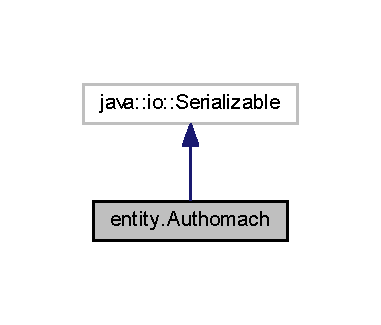
\includegraphics[width=183pt]{classentity_1_1_authomach__inherit__graph}
\end{center}
\end{figure}


Collaboration diagram for entity.\+Authomach\+:\nopagebreak
\begin{figure}[H]
\begin{center}
\leavevmode
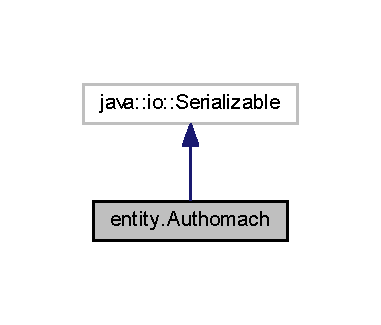
\includegraphics[width=183pt]{classentity_1_1_authomach__coll__graph}
\end{center}
\end{figure}
\subsection*{Public Member Functions}
\begin{DoxyCompactItemize}
\item 
\mbox{\Hypertarget{classentity_1_1_authomach_a8f9bf217f1a51601009ce0da96571cf2}\label{classentity_1_1_authomach_a8f9bf217f1a51601009ce0da96571cf2}} 
{\bfseries Authomach} (String description, Boolean state, Set carrieses)
\item 
\mbox{\Hypertarget{classentity_1_1_authomach_aa123815d3d8c471756c298edba10d4e1}\label{classentity_1_1_authomach_aa123815d3d8c471756c298edba10d4e1}} 
int {\bfseries get\+Machine\+Id} ()
\item 
\mbox{\Hypertarget{classentity_1_1_authomach_aa7eb52c9c1828f6870b84727cb2fd7d9}\label{classentity_1_1_authomach_aa7eb52c9c1828f6870b84727cb2fd7d9}} 
void {\bfseries set\+Machine\+Id} (int machine\+Id)
\item 
\mbox{\Hypertarget{classentity_1_1_authomach_ac935bc6cd52b576e53a3f58c6bb1eb1e}\label{classentity_1_1_authomach_ac935bc6cd52b576e53a3f58c6bb1eb1e}} 
String {\bfseries get\+Description} ()
\item 
\mbox{\Hypertarget{classentity_1_1_authomach_ab49dd6d37693e9b4a32e881aae5ec898}\label{classentity_1_1_authomach_ab49dd6d37693e9b4a32e881aae5ec898}} 
void {\bfseries set\+Description} (String description)
\item 
\mbox{\Hypertarget{classentity_1_1_authomach_a6c2b7c4d9aeb91c62791854f9f472b89}\label{classentity_1_1_authomach_a6c2b7c4d9aeb91c62791854f9f472b89}} 
Boolean {\bfseries get\+State} ()
\item 
\mbox{\Hypertarget{classentity_1_1_authomach_a7efa67cff55a9d3678745f918a26d7c8}\label{classentity_1_1_authomach_a7efa67cff55a9d3678745f918a26d7c8}} 
void {\bfseries set\+State} (Boolean state)
\end{DoxyCompactItemize}


\subsection{Detailed Description}
\mbox{\hyperlink{classentity_1_1_authomach}{Authomach}} generated by hbm2java 

The documentation for this class was generated from the following file\+:\begin{DoxyCompactItemize}
\item 
src/main/java/entity/Authomach.\+java\end{DoxyCompactItemize}

\hypertarget{classentity_1_1copy_1_1_authomach}{}\section{entity.\+copy.\+Authomach Class Reference}
\label{classentity_1_1copy_1_1_authomach}\index{entity.\+copy.\+Authomach@{entity.\+copy.\+Authomach}}


Inheritance diagram for entity.\+copy.\+Authomach\+:
% FIG 0


Collaboration diagram for entity.\+copy.\+Authomach\+:
% FIG 1
\subsection*{Public Member Functions}
\begin{DoxyCompactItemize}
\item 
\mbox{\Hypertarget{classentity_1_1copy_1_1_authomach_a3e349d7d48beaeb7f0601235f605c639}\label{classentity_1_1copy_1_1_authomach_a3e349d7d48beaeb7f0601235f605c639}} 
{\bfseries Authomach} (String machine)
\item 
\mbox{\Hypertarget{classentity_1_1copy_1_1_authomach_ac8ff6c70f01e96099a69ebcc0b378be5}\label{classentity_1_1copy_1_1_authomach_ac8ff6c70f01e96099a69ebcc0b378be5}} 
{\bfseries Authomach} (\mbox{\hyperlink{classentity_1_1copy_1_1_segment}{Segment}} segment, String machine, String description, Boolean state, Set carrieses)
\item 
\mbox{\Hypertarget{classentity_1_1copy_1_1_authomach_a58cc53cd5750a5cdbe1285f09adb7789}\label{classentity_1_1copy_1_1_authomach_a58cc53cd5750a5cdbe1285f09adb7789}} 
int {\bfseries get\+Machine\+Id} ()
\item 
\mbox{\Hypertarget{classentity_1_1copy_1_1_authomach_a2f759faf41a0fe3d47c668272f4bf51c}\label{classentity_1_1copy_1_1_authomach_a2f759faf41a0fe3d47c668272f4bf51c}} 
void {\bfseries set\+Machine\+Id} (int machine\+Id)
\item 
\mbox{\Hypertarget{classentity_1_1copy_1_1_authomach_a6920deffc9abe3959051b3bcd7646109}\label{classentity_1_1copy_1_1_authomach_a6920deffc9abe3959051b3bcd7646109}} 
\mbox{\hyperlink{classentity_1_1copy_1_1_segment}{Segment}} {\bfseries get\+Segment} ()
\item 
\mbox{\Hypertarget{classentity_1_1copy_1_1_authomach_a68a60a7503bd412900005d906e1705c5}\label{classentity_1_1copy_1_1_authomach_a68a60a7503bd412900005d906e1705c5}} 
void {\bfseries set\+Segment} (\mbox{\hyperlink{classentity_1_1copy_1_1_segment}{Segment}} segment)
\item 
\mbox{\Hypertarget{classentity_1_1copy_1_1_authomach_a360be33d879aae5e3fbb859c796b44b8}\label{classentity_1_1copy_1_1_authomach_a360be33d879aae5e3fbb859c796b44b8}} 
String {\bfseries get\+Machine} ()
\item 
\mbox{\Hypertarget{classentity_1_1copy_1_1_authomach_a416244e1374670a0f9399e7010dc07e0}\label{classentity_1_1copy_1_1_authomach_a416244e1374670a0f9399e7010dc07e0}} 
void {\bfseries set\+Machine} (String machine)
\item 
\mbox{\Hypertarget{classentity_1_1copy_1_1_authomach_a615a9608fba84c4c8b90976c23d63586}\label{classentity_1_1copy_1_1_authomach_a615a9608fba84c4c8b90976c23d63586}} 
String {\bfseries get\+Description} ()
\item 
\mbox{\Hypertarget{classentity_1_1copy_1_1_authomach_abe84ee8ba1e2df0f8c818bb92652d9ce}\label{classentity_1_1copy_1_1_authomach_abe84ee8ba1e2df0f8c818bb92652d9ce}} 
void {\bfseries set\+Description} (String description)
\item 
\mbox{\Hypertarget{classentity_1_1copy_1_1_authomach_ac23c04925ebda9994235b16790921776}\label{classentity_1_1copy_1_1_authomach_ac23c04925ebda9994235b16790921776}} 
Boolean {\bfseries get\+State} ()
\item 
\mbox{\Hypertarget{classentity_1_1copy_1_1_authomach_a28335b1654f0e0f618c370a26a4534c9}\label{classentity_1_1copy_1_1_authomach_a28335b1654f0e0f618c370a26a4534c9}} 
void {\bfseries set\+State} (Boolean state)
\item 
\mbox{\Hypertarget{classentity_1_1copy_1_1_authomach_a09a43e7c6e2261338ff4525792ad3293}\label{classentity_1_1copy_1_1_authomach_a09a43e7c6e2261338ff4525792ad3293}} 
Set {\bfseries get\+Carrieses} ()
\item 
\mbox{\Hypertarget{classentity_1_1copy_1_1_authomach_a252f59dee99ca828f6e5ee93c08d9a7e}\label{classentity_1_1copy_1_1_authomach_a252f59dee99ca828f6e5ee93c08d9a7e}} 
void {\bfseries set\+Carrieses} (Set carrieses)
\end{DoxyCompactItemize}


\subsection{Detailed Description}
\mbox{\hyperlink{classentity_1_1copy_1_1_authomach}{Authomach}} generated by hbm2java 

The documentation for this class was generated from the following file\+:\begin{DoxyCompactItemize}
\item 
D\+:/\+Users/user/\+Documents/\+M\+O\+N\+D\+R\+A/3.\+M\+A\+I\+L\+A/\+P\+O\+P\+B\+L5/\+G\+I\+T/e\+Jkiva\+\_\+\+P\+O\+P\+B\+L5/e\+Jkiva/src/main/java/entity/copy/Authomach.\+java\end{DoxyCompactItemize}

\hypertarget{classentity_1_1copy_1_1_carries}{}\section{entity.\+copy.\+Carries Class Reference}
\label{classentity_1_1copy_1_1_carries}\index{entity.\+copy.\+Carries@{entity.\+copy.\+Carries}}


Inheritance diagram for entity.\+copy.\+Carries\+:
% FIG 0


Collaboration diagram for entity.\+copy.\+Carries\+:
% FIG 1
\subsection*{Public Member Functions}
\begin{DoxyCompactItemize}
\item 
\mbox{\Hypertarget{classentity_1_1copy_1_1_carries_aeaec16c60fb4f88a6d0e3a96cb98d68d}\label{classentity_1_1copy_1_1_carries_aeaec16c60fb4f88a6d0e3a96cb98d68d}} 
{\bfseries Carries} (\mbox{\hyperlink{classentity_1_1copy_1_1_carries_id}{Carries\+Id}} id, \mbox{\hyperlink{classentity_1_1copy_1_1_orderproduct}{Orderproduct}} orderproduct)
\item 
\mbox{\Hypertarget{classentity_1_1copy_1_1_carries_ae3456ca921defd8681c6d49fb8c62e83}\label{classentity_1_1copy_1_1_carries_ae3456ca921defd8681c6d49fb8c62e83}} 
{\bfseries Carries} (\mbox{\hyperlink{classentity_1_1copy_1_1_carries_id}{Carries\+Id}} id, \mbox{\hyperlink{classentity_1_1copy_1_1_authomach}{Authomach}} authomach, \mbox{\hyperlink{classentity_1_1copy_1_1_orderproduct}{Orderproduct}} orderproduct, \mbox{\hyperlink{classentity_1_1copy_1_1_workstation}{Workstation}} workstation\+By\+Destiny\+Workstation\+Id, \mbox{\hyperlink{classentity_1_1copy_1_1_workstation}{Workstation}} workstation\+By\+Initial\+Workstation\+Id)
\item 
\mbox{\Hypertarget{classentity_1_1copy_1_1_carries_ad43a95853c171a2bb2cf36c3bd3d5120}\label{classentity_1_1copy_1_1_carries_ad43a95853c171a2bb2cf36c3bd3d5120}} 
\mbox{\hyperlink{classentity_1_1copy_1_1_carries_id}{Carries\+Id}} {\bfseries get\+Id} ()
\item 
\mbox{\Hypertarget{classentity_1_1copy_1_1_carries_a61b5a3743df6e27848fd70b53009fb77}\label{classentity_1_1copy_1_1_carries_a61b5a3743df6e27848fd70b53009fb77}} 
void {\bfseries set\+Id} (\mbox{\hyperlink{classentity_1_1copy_1_1_carries_id}{Carries\+Id}} id)
\item 
\mbox{\Hypertarget{classentity_1_1copy_1_1_carries_a0ec3f603cbeacaa2b432a185d736fd62}\label{classentity_1_1copy_1_1_carries_a0ec3f603cbeacaa2b432a185d736fd62}} 
\mbox{\hyperlink{classentity_1_1copy_1_1_authomach}{Authomach}} {\bfseries get\+Authomach} ()
\item 
\mbox{\Hypertarget{classentity_1_1copy_1_1_carries_a649bdb4de46f63fb4b109256593aab95}\label{classentity_1_1copy_1_1_carries_a649bdb4de46f63fb4b109256593aab95}} 
void {\bfseries set\+Authomach} (\mbox{\hyperlink{classentity_1_1copy_1_1_authomach}{Authomach}} authomach)
\item 
\mbox{\Hypertarget{classentity_1_1copy_1_1_carries_a81468014f97e67fb9d8bce8f75321d42}\label{classentity_1_1copy_1_1_carries_a81468014f97e67fb9d8bce8f75321d42}} 
\mbox{\hyperlink{classentity_1_1copy_1_1_orderproduct}{Orderproduct}} {\bfseries get\+Orderproduct} ()
\item 
\mbox{\Hypertarget{classentity_1_1copy_1_1_carries_ab6a366911005a8372e3b64c0155fbfd0}\label{classentity_1_1copy_1_1_carries_ab6a366911005a8372e3b64c0155fbfd0}} 
void {\bfseries set\+Orderproduct} (\mbox{\hyperlink{classentity_1_1copy_1_1_orderproduct}{Orderproduct}} orderproduct)
\item 
\mbox{\Hypertarget{classentity_1_1copy_1_1_carries_a322871db33089a7efbec3b19d3507f4e}\label{classentity_1_1copy_1_1_carries_a322871db33089a7efbec3b19d3507f4e}} 
\mbox{\hyperlink{classentity_1_1copy_1_1_workstation}{Workstation}} {\bfseries get\+Workstation\+By\+Destiny\+Workstation\+Id} ()
\item 
\mbox{\Hypertarget{classentity_1_1copy_1_1_carries_a454e92311cac2b97ef80b17effad2405}\label{classentity_1_1copy_1_1_carries_a454e92311cac2b97ef80b17effad2405}} 
void {\bfseries set\+Workstation\+By\+Destiny\+Workstation\+Id} (\mbox{\hyperlink{classentity_1_1copy_1_1_workstation}{Workstation}} workstation\+By\+Destiny\+Workstation\+Id)
\item 
\mbox{\Hypertarget{classentity_1_1copy_1_1_carries_a0e468ba3806ccbe3d466b84d1d0c292f}\label{classentity_1_1copy_1_1_carries_a0e468ba3806ccbe3d466b84d1d0c292f}} 
\mbox{\hyperlink{classentity_1_1copy_1_1_workstation}{Workstation}} {\bfseries get\+Workstation\+By\+Initial\+Workstation\+Id} ()
\item 
\mbox{\Hypertarget{classentity_1_1copy_1_1_carries_a49fe6fe16889c3ef8d7ab6fbd49bc25f}\label{classentity_1_1copy_1_1_carries_a49fe6fe16889c3ef8d7ab6fbd49bc25f}} 
void {\bfseries set\+Workstation\+By\+Initial\+Workstation\+Id} (\mbox{\hyperlink{classentity_1_1copy_1_1_workstation}{Workstation}} workstation\+By\+Initial\+Workstation\+Id)
\end{DoxyCompactItemize}


\subsection{Detailed Description}
\mbox{\hyperlink{classentity_1_1copy_1_1_carries}{Carries}} generated by hbm2java 

The documentation for this class was generated from the following file\+:\begin{DoxyCompactItemize}
\item 
D\+:/\+Users/user/\+Documents/\+M\+O\+N\+D\+R\+A/3.\+M\+A\+I\+L\+A/\+P\+O\+P\+B\+L5/\+G\+I\+T/e\+Jkiva\+\_\+\+P\+O\+P\+B\+L5/e\+Jkiva/src/main/java/entity/copy/Carries.\+java\end{DoxyCompactItemize}

\hypertarget{classentity_1_1_carries}{}\section{entity.\+Carries Class Reference}
\label{classentity_1_1_carries}\index{entity.\+Carries@{entity.\+Carries}}


Inheritance diagram for entity.\+Carries\+:\nopagebreak
\begin{figure}[H]
\begin{center}
\leavevmode
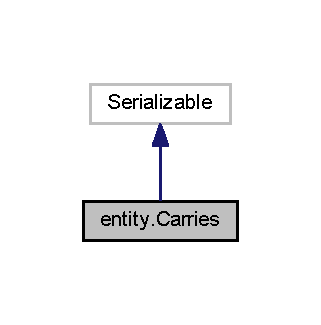
\includegraphics[width=154pt]{classentity_1_1_carries__inherit__graph}
\end{center}
\end{figure}


Collaboration diagram for entity.\+Carries\+:\nopagebreak
\begin{figure}[H]
\begin{center}
\leavevmode
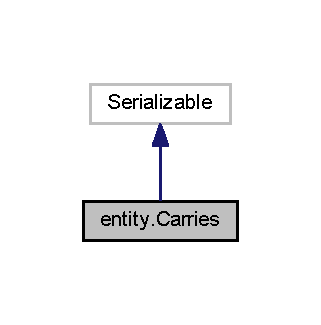
\includegraphics[width=154pt]{classentity_1_1_carries__coll__graph}
\end{center}
\end{figure}
\subsection*{Public Member Functions}
\begin{DoxyCompactItemize}
\item 
\mbox{\Hypertarget{classentity_1_1_carries_acf6db6a8bebc1383fb44b5d1a69db994}\label{classentity_1_1_carries_acf6db6a8bebc1383fb44b5d1a69db994}} 
{\bfseries Carries} (\mbox{\hyperlink{classentity_1_1_carries_id}{Carries\+Id}} id, \mbox{\hyperlink{classentity_1_1_orderproduct}{Orderproduct}} orderproduct)
\item 
\mbox{\Hypertarget{classentity_1_1_carries_a61138413c175da3c338dd6d3faf5034d}\label{classentity_1_1_carries_a61138413c175da3c338dd6d3faf5034d}} 
{\bfseries Carries} (\mbox{\hyperlink{classentity_1_1_carries_id}{Carries\+Id}} id, \mbox{\hyperlink{classentity_1_1_authomach}{Authomach}} authomach, \mbox{\hyperlink{classentity_1_1_orderproduct}{Orderproduct}} orderproduct, \mbox{\hyperlink{classentity_1_1_workstation}{Workstation}} workstation\+By\+Destiny\+Workstation\+Id, \mbox{\hyperlink{classentity_1_1_workstation}{Workstation}} workstation\+By\+Initial\+Workstation\+Id)
\item 
\mbox{\Hypertarget{classentity_1_1_carries_af1a678cc4d0ded3e9fecbf0a17a2ba3c}\label{classentity_1_1_carries_af1a678cc4d0ded3e9fecbf0a17a2ba3c}} 
\mbox{\hyperlink{classentity_1_1_carries_id}{Carries\+Id}} {\bfseries get\+Id} ()
\item 
\mbox{\Hypertarget{classentity_1_1_carries_a23d2ab3f05610f37bca03e7cc08ced73}\label{classentity_1_1_carries_a23d2ab3f05610f37bca03e7cc08ced73}} 
void {\bfseries set\+Id} (\mbox{\hyperlink{classentity_1_1_carries_id}{Carries\+Id}} id)
\item 
\mbox{\Hypertarget{classentity_1_1_carries_a539e6149274e7be94d86999d02af82d1}\label{classentity_1_1_carries_a539e6149274e7be94d86999d02af82d1}} 
\mbox{\hyperlink{classentity_1_1_authomach}{Authomach}} {\bfseries get\+Authomach} ()
\item 
\mbox{\Hypertarget{classentity_1_1_carries_a5fddad71e78d3206116e710916c8bb74}\label{classentity_1_1_carries_a5fddad71e78d3206116e710916c8bb74}} 
void {\bfseries set\+Authomach} (\mbox{\hyperlink{classentity_1_1_authomach}{Authomach}} authomach)
\item 
\mbox{\Hypertarget{classentity_1_1_carries_a6439c3d458849f3f5d87c0f9577fc16b}\label{classentity_1_1_carries_a6439c3d458849f3f5d87c0f9577fc16b}} 
\mbox{\hyperlink{classentity_1_1_orderproduct}{Orderproduct}} {\bfseries get\+Orderproduct} ()
\item 
\mbox{\Hypertarget{classentity_1_1_carries_af3856ed5dc8866063ed552e5a6289736}\label{classentity_1_1_carries_af3856ed5dc8866063ed552e5a6289736}} 
void {\bfseries set\+Orderproduct} (\mbox{\hyperlink{classentity_1_1_orderproduct}{Orderproduct}} orderproduct)
\item 
\mbox{\Hypertarget{classentity_1_1_carries_a13e9ee65fee8f33abd1b5fcd4da046c2}\label{classentity_1_1_carries_a13e9ee65fee8f33abd1b5fcd4da046c2}} 
\mbox{\hyperlink{classentity_1_1_workstation}{Workstation}} {\bfseries get\+Workstation\+By\+Destiny\+Workstation\+Id} ()
\item 
\mbox{\Hypertarget{classentity_1_1_carries_a97c1c2cb313a25a61f86e538345ae58f}\label{classentity_1_1_carries_a97c1c2cb313a25a61f86e538345ae58f}} 
void {\bfseries set\+Workstation\+By\+Destiny\+Workstation\+Id} (\mbox{\hyperlink{classentity_1_1_workstation}{Workstation}} workstation\+By\+Destiny\+Workstation\+Id)
\item 
\mbox{\Hypertarget{classentity_1_1_carries_a4d75d589a3902ef133f3be58d725b852}\label{classentity_1_1_carries_a4d75d589a3902ef133f3be58d725b852}} 
\mbox{\hyperlink{classentity_1_1_workstation}{Workstation}} {\bfseries get\+Workstation\+By\+Initial\+Workstation\+Id} ()
\item 
\mbox{\Hypertarget{classentity_1_1_carries_a807fe564289f14063a30047d3cea3522}\label{classentity_1_1_carries_a807fe564289f14063a30047d3cea3522}} 
void {\bfseries set\+Workstation\+By\+Initial\+Workstation\+Id} (\mbox{\hyperlink{classentity_1_1_workstation}{Workstation}} workstation\+By\+Initial\+Workstation\+Id)
\end{DoxyCompactItemize}


\subsection{Detailed Description}
\mbox{\hyperlink{classentity_1_1_carries}{Carries}} generated by hbm2java 

The documentation for this class was generated from the following file\+:\begin{DoxyCompactItemize}
\item 
src/main/java/entity/Carries.\+java\end{DoxyCompactItemize}

\hypertarget{classentity_1_1copy_1_1_carries_id}{}\section{entity.\+copy.\+Carries\+Id Class Reference}
\label{classentity_1_1copy_1_1_carries_id}\index{entity.\+copy.\+Carries\+Id@{entity.\+copy.\+Carries\+Id}}


Inheritance diagram for entity.\+copy.\+Carries\+Id\+:
% FIG 0


Collaboration diagram for entity.\+copy.\+Carries\+Id\+:
% FIG 1
\subsection*{Public Member Functions}
\begin{DoxyCompactItemize}
\item 
\mbox{\Hypertarget{classentity_1_1copy_1_1_carries_id_aed584e777849953ca686b1ed2ec249d1}\label{classentity_1_1copy_1_1_carries_id_aed584e777849953ca686b1ed2ec249d1}} 
{\bfseries Carries\+Id} (byte order\+Product\+Id)
\item 
\mbox{\Hypertarget{classentity_1_1copy_1_1_carries_id_a3adc4e3947e439c8c23b9e91a68de5aa}\label{classentity_1_1copy_1_1_carries_id_a3adc4e3947e439c8c23b9e91a68de5aa}} 
{\bfseries Carries\+Id} (byte order\+Product\+Id, Byte initial\+Workstation\+Id, Byte destiny\+Workstation\+Id, Byte machine\+Id, Boolean state)
\item 
\mbox{\Hypertarget{classentity_1_1copy_1_1_carries_id_ae26aa1ca3dc654b2c255a004c493b47d}\label{classentity_1_1copy_1_1_carries_id_ae26aa1ca3dc654b2c255a004c493b47d}} 
int {\bfseries get\+Order\+Product\+Id} ()
\item 
\mbox{\Hypertarget{classentity_1_1copy_1_1_carries_id_a074d02bc965f66a407a4aa8780c06b97}\label{classentity_1_1copy_1_1_carries_id_a074d02bc965f66a407a4aa8780c06b97}} 
void {\bfseries set\+Order\+Product\+Id} (int order\+Product\+Id)
\item 
\mbox{\Hypertarget{classentity_1_1copy_1_1_carries_id_acd710775871c86cf48f0c93a4af87779}\label{classentity_1_1copy_1_1_carries_id_acd710775871c86cf48f0c93a4af87779}} 
Byte {\bfseries get\+Initial\+Workstation\+Id} ()
\item 
\mbox{\Hypertarget{classentity_1_1copy_1_1_carries_id_abbdc0b1d8993920dc1a582bf6757b51a}\label{classentity_1_1copy_1_1_carries_id_abbdc0b1d8993920dc1a582bf6757b51a}} 
void {\bfseries set\+Initial\+Workstation\+Id} (Byte initial\+Workstation\+Id)
\item 
\mbox{\Hypertarget{classentity_1_1copy_1_1_carries_id_a3b92926f9d7d04700658a2ca09c1949b}\label{classentity_1_1copy_1_1_carries_id_a3b92926f9d7d04700658a2ca09c1949b}} 
Byte {\bfseries get\+Destiny\+Workstation\+Id} ()
\item 
\mbox{\Hypertarget{classentity_1_1copy_1_1_carries_id_af2e185e73b174cecc828ff9f37e2adcb}\label{classentity_1_1copy_1_1_carries_id_af2e185e73b174cecc828ff9f37e2adcb}} 
void {\bfseries set\+Destiny\+Workstation\+Id} (Byte destiny\+Workstation\+Id)
\item 
\mbox{\Hypertarget{classentity_1_1copy_1_1_carries_id_a49ff35e89fb8daa8ba192018570a9943}\label{classentity_1_1copy_1_1_carries_id_a49ff35e89fb8daa8ba192018570a9943}} 
Byte {\bfseries get\+Machine\+Id} ()
\item 
\mbox{\Hypertarget{classentity_1_1copy_1_1_carries_id_adf6dfc721ab97c887eff0950c6d96cf5}\label{classentity_1_1copy_1_1_carries_id_adf6dfc721ab97c887eff0950c6d96cf5}} 
void {\bfseries set\+Machine\+Id} (Byte machine\+Id)
\item 
\mbox{\Hypertarget{classentity_1_1copy_1_1_carries_id_a7756055589896e6afd6e8310afa760a8}\label{classentity_1_1copy_1_1_carries_id_a7756055589896e6afd6e8310afa760a8}} 
Boolean {\bfseries get\+State} ()
\item 
\mbox{\Hypertarget{classentity_1_1copy_1_1_carries_id_aac9c996ac0331aa86aca3c99563c60a1}\label{classentity_1_1copy_1_1_carries_id_aac9c996ac0331aa86aca3c99563c60a1}} 
void {\bfseries set\+State} (Boolean state)
\item 
\mbox{\Hypertarget{classentity_1_1copy_1_1_carries_id_a0975b7c3dfab07c82b06b04efdce801f}\label{classentity_1_1copy_1_1_carries_id_a0975b7c3dfab07c82b06b04efdce801f}} 
boolean {\bfseries equals} (Object other)
\item 
\mbox{\Hypertarget{classentity_1_1copy_1_1_carries_id_afa655532570f3accf87116cea68afa61}\label{classentity_1_1copy_1_1_carries_id_afa655532570f3accf87116cea68afa61}} 
int {\bfseries hash\+Code} ()
\end{DoxyCompactItemize}


\subsection{Detailed Description}
\mbox{\hyperlink{classentity_1_1copy_1_1_carries_id}{Carries\+Id}} generated by hbm2java 

The documentation for this class was generated from the following file\+:\begin{DoxyCompactItemize}
\item 
D\+:/\+Users/user/\+Documents/\+M\+O\+N\+D\+R\+A/3.\+M\+A\+I\+L\+A/\+P\+O\+P\+B\+L5/\+G\+I\+T/e\+Jkiva\+\_\+\+P\+O\+P\+B\+L5/e\+Jkiva/src/main/java/entity/copy/Carries\+Id.\+java\end{DoxyCompactItemize}

\hypertarget{classentity_1_1_carries_id}{}\section{entity.\+Carries\+Id Class Reference}
\label{classentity_1_1_carries_id}\index{entity.\+Carries\+Id@{entity.\+Carries\+Id}}


Inheritance diagram for entity.\+Carries\+Id\+:\nopagebreak
\begin{figure}[H]
\begin{center}
\leavevmode
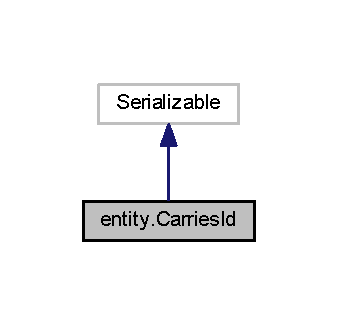
\includegraphics[width=162pt]{classentity_1_1_carries_id__inherit__graph}
\end{center}
\end{figure}


Collaboration diagram for entity.\+Carries\+Id\+:\nopagebreak
\begin{figure}[H]
\begin{center}
\leavevmode
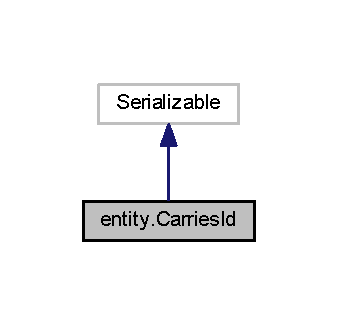
\includegraphics[width=162pt]{classentity_1_1_carries_id__coll__graph}
\end{center}
\end{figure}
\subsection*{Public Member Functions}
\begin{DoxyCompactItemize}
\item 
\mbox{\Hypertarget{classentity_1_1_carries_id_a51dae5e60540dcdb4b5c4a5c59ce8aed}\label{classentity_1_1_carries_id_a51dae5e60540dcdb4b5c4a5c59ce8aed}} 
{\bfseries Carries\+Id} (byte order\+Product\+Id)
\item 
\mbox{\Hypertarget{classentity_1_1_carries_id_a3c7555deb455253a857ecb72a99c0c1e}\label{classentity_1_1_carries_id_a3c7555deb455253a857ecb72a99c0c1e}} 
{\bfseries Carries\+Id} (byte order\+Product\+Id, Byte initial\+Workstation\+Id, Byte destiny\+Workstation\+Id, Byte machine\+Id, Boolean state)
\item 
\mbox{\Hypertarget{classentity_1_1_carries_id_a774d57bdffd816d281e67bd06bf62d21}\label{classentity_1_1_carries_id_a774d57bdffd816d281e67bd06bf62d21}} 
int {\bfseries get\+Order\+Product\+Id} ()
\item 
\mbox{\Hypertarget{classentity_1_1_carries_id_a9049878112d9a3423f96ea5593afeb6f}\label{classentity_1_1_carries_id_a9049878112d9a3423f96ea5593afeb6f}} 
void {\bfseries set\+Order\+Product\+Id} (int order\+Product\+Id)
\item 
\mbox{\Hypertarget{classentity_1_1_carries_id_a9f0d4a30dbe0db09bab463393bd6d1f5}\label{classentity_1_1_carries_id_a9f0d4a30dbe0db09bab463393bd6d1f5}} 
Byte {\bfseries get\+Initial\+Workstation\+Id} ()
\item 
\mbox{\Hypertarget{classentity_1_1_carries_id_a2f055c85f701e12e2d93e054189414c6}\label{classentity_1_1_carries_id_a2f055c85f701e12e2d93e054189414c6}} 
void {\bfseries set\+Initial\+Workstation\+Id} (Byte initial\+Workstation\+Id)
\item 
\mbox{\Hypertarget{classentity_1_1_carries_id_a6806d0507a1e0e67cc2cb3668255a1b8}\label{classentity_1_1_carries_id_a6806d0507a1e0e67cc2cb3668255a1b8}} 
Byte {\bfseries get\+Destiny\+Workstation\+Id} ()
\item 
\mbox{\Hypertarget{classentity_1_1_carries_id_af9516f9d5e88954e3e72457f2ccf4f7b}\label{classentity_1_1_carries_id_af9516f9d5e88954e3e72457f2ccf4f7b}} 
void {\bfseries set\+Destiny\+Workstation\+Id} (Byte destiny\+Workstation\+Id)
\item 
\mbox{\Hypertarget{classentity_1_1_carries_id_a625fe262ed6c802bc07f9f4cc4a989bb}\label{classentity_1_1_carries_id_a625fe262ed6c802bc07f9f4cc4a989bb}} 
Byte {\bfseries get\+Machine\+Id} ()
\item 
\mbox{\Hypertarget{classentity_1_1_carries_id_aa5bba6ca3cb097ea91354987f1b6a2f0}\label{classentity_1_1_carries_id_aa5bba6ca3cb097ea91354987f1b6a2f0}} 
void {\bfseries set\+Machine\+Id} (Byte machine\+Id)
\item 
\mbox{\Hypertarget{classentity_1_1_carries_id_a123b2805042dd0fe551c2e766b961129}\label{classentity_1_1_carries_id_a123b2805042dd0fe551c2e766b961129}} 
Boolean {\bfseries get\+State} ()
\item 
\mbox{\Hypertarget{classentity_1_1_carries_id_a8f8f0f103d2fd8db15b6416370d690e1}\label{classentity_1_1_carries_id_a8f8f0f103d2fd8db15b6416370d690e1}} 
void {\bfseries set\+State} (Boolean state)
\item 
\mbox{\Hypertarget{classentity_1_1_carries_id_ac343763b0821ae53aa653fc269cb0172}\label{classentity_1_1_carries_id_ac343763b0821ae53aa653fc269cb0172}} 
boolean {\bfseries equals} (Object other)
\item 
\mbox{\Hypertarget{classentity_1_1_carries_id_a2d5ebee74ab620ab24e2ab3da501cfd9}\label{classentity_1_1_carries_id_a2d5ebee74ab620ab24e2ab3da501cfd9}} 
int {\bfseries hash\+Code} ()
\end{DoxyCompactItemize}


\subsection{Detailed Description}
\mbox{\hyperlink{classentity_1_1_carries_id}{Carries\+Id}} generated by hbm2java 

The documentation for this class was generated from the following file\+:\begin{DoxyCompactItemize}
\item 
src/main/java/entity/Carries\+Id.\+java\end{DoxyCompactItemize}

\hypertarget{classcontroller_1_1_customer_controller}{}\section{controller.\+Customer\+Controller Class Reference}
\label{classcontroller_1_1_customer_controller}\index{controller.\+Customer\+Controller@{controller.\+Customer\+Controller}}


Collaboration diagram for controller.\+Customer\+Controller\+:\nopagebreak
\begin{figure}[H]
\begin{center}
\leavevmode
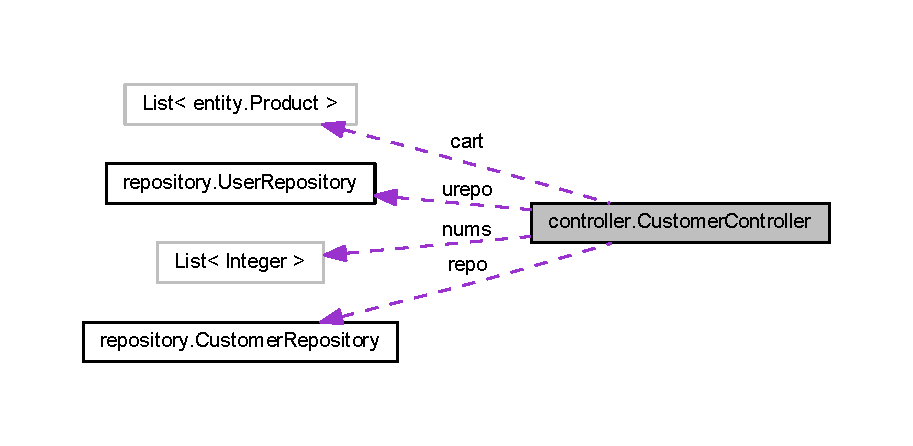
\includegraphics[width=350pt]{classcontroller_1_1_customer_controller__coll__graph}
\end{center}
\end{figure}
\subsection*{Public Member Functions}
\begin{DoxyCompactItemize}
\item 
String \mbox{\hyperlink{classcontroller_1_1_customer_controller_a5496f4bf5f03f585ee223c0192d4fc85}{customer}} (Model m, Web\+Request request, Http\+Servlet\+Response response, Http\+Servlet\+Request hrequest)  throws I\+O\+Exception 
\item 
String \mbox{\hyperlink{classcontroller_1_1_customer_controller_a9c7aebe2a5ae4e7419fd10121a6a7189}{show\+Product}} (Model m, Web\+Request request, Http\+Servlet\+Response response, Http\+Servlet\+Request hrequest)  throws I\+O\+Exception 
\item 
String \mbox{\hyperlink{classcontroller_1_1_customer_controller_af47f965b533083f4415c63f1065cbd64}{orders}} (Model m, Web\+Request request, Http\+Servlet\+Request hrequest, Http\+Servlet\+Response response)  throws I\+O\+Exception 
\item 
String \mbox{\hyperlink{classcontroller_1_1_customer_controller_a74ff447f25dce313f84a08cf5356f8e8}{order}} (Model m, Web\+Request request)
\item 
String \mbox{\hyperlink{classcontroller_1_1_customer_controller_a90aa906ff9e90be62b82941992350235}{cart}} (Model m, Web\+Request request, Http\+Servlet\+Request hrequest, Http\+Servlet\+Response response)  throws I\+O\+Exception 
\item 
String \mbox{\hyperlink{classcontroller_1_1_customer_controller_add866b64d6e08876db8b97087eaeb389}{chart}} (Model m, Web\+Request request)
\end{DoxyCompactItemize}


\subsection{Detailed Description}
\mbox{\hyperlink{classcontroller_1_1_customer_controller}{Customer\+Controller}} contains the U\+RL actions of the Customer user type

\begin{DoxyAuthor}{Author}
Leire 
\end{DoxyAuthor}


\subsection{Member Function Documentation}
\mbox{\Hypertarget{classcontroller_1_1_customer_controller_a90aa906ff9e90be62b82941992350235}\label{classcontroller_1_1_customer_controller_a90aa906ff9e90be62b82941992350235}} 
\index{controller\+::\+Customer\+Controller@{controller\+::\+Customer\+Controller}!cart@{cart}}
\index{cart@{cart}!controller\+::\+Customer\+Controller@{controller\+::\+Customer\+Controller}}
\subsubsection{\texorpdfstring{cart()}{cart()}}
{\footnotesize\ttfamily String controller.\+Customer\+Controller.\+cart (\begin{DoxyParamCaption}\item[{Model}]{m,  }\item[{Web\+Request}]{request,  }\item[{Http\+Servlet\+Request}]{hrequest,  }\item[{Http\+Servlet\+Response}]{response }\end{DoxyParamCaption}) throws I\+O\+Exception\hspace{0.3cm}{\ttfamily [inline]}}

This method will show the actual cart of the customer 
\begin{DoxyExceptions}{Exceptions}
{\em I\+O\+Exception} & \\
\hline
\end{DoxyExceptions}
\mbox{\Hypertarget{classcontroller_1_1_customer_controller_add866b64d6e08876db8b97087eaeb389}\label{classcontroller_1_1_customer_controller_add866b64d6e08876db8b97087eaeb389}} 
\index{controller\+::\+Customer\+Controller@{controller\+::\+Customer\+Controller}!chart@{chart}}
\index{chart@{chart}!controller\+::\+Customer\+Controller@{controller\+::\+Customer\+Controller}}
\subsubsection{\texorpdfstring{chart()}{chart()}}
{\footnotesize\ttfamily String controller.\+Customer\+Controller.\+chart (\begin{DoxyParamCaption}\item[{Model}]{m,  }\item[{Web\+Request}]{request }\end{DoxyParamCaption})\hspace{0.3cm}{\ttfamily [inline]}}

This method will show a chart showing the history of the products bought by the customer \mbox{\Hypertarget{classcontroller_1_1_customer_controller_a5496f4bf5f03f585ee223c0192d4fc85}\label{classcontroller_1_1_customer_controller_a5496f4bf5f03f585ee223c0192d4fc85}} 
\index{controller\+::\+Customer\+Controller@{controller\+::\+Customer\+Controller}!customer@{customer}}
\index{customer@{customer}!controller\+::\+Customer\+Controller@{controller\+::\+Customer\+Controller}}
\subsubsection{\texorpdfstring{customer()}{customer()}}
{\footnotesize\ttfamily String controller.\+Customer\+Controller.\+customer (\begin{DoxyParamCaption}\item[{Model}]{m,  }\item[{Web\+Request}]{request,  }\item[{Http\+Servlet\+Response}]{response,  }\item[{Http\+Servlet\+Request}]{hrequest }\end{DoxyParamCaption}) throws I\+O\+Exception\hspace{0.3cm}{\ttfamily [inline]}}

This method will access the customer\textquotesingle{}s main site. Here, the customer will be able to see all the products available on the store. 
\begin{DoxyExceptions}{Exceptions}
{\em I\+O\+Exception} & \\
\hline
\end{DoxyExceptions}
\mbox{\Hypertarget{classcontroller_1_1_customer_controller_a74ff447f25dce313f84a08cf5356f8e8}\label{classcontroller_1_1_customer_controller_a74ff447f25dce313f84a08cf5356f8e8}} 
\index{controller\+::\+Customer\+Controller@{controller\+::\+Customer\+Controller}!order@{order}}
\index{order@{order}!controller\+::\+Customer\+Controller@{controller\+::\+Customer\+Controller}}
\subsubsection{\texorpdfstring{order()}{order()}}
{\footnotesize\ttfamily String controller.\+Customer\+Controller.\+order (\begin{DoxyParamCaption}\item[{Model}]{m,  }\item[{Web\+Request}]{request }\end{DoxyParamCaption})\hspace{0.3cm}{\ttfamily [inline]}}

This method will access the customer\textquotesingle{}s \textquotesingle{}orders\textquotesingle{} option, where the customer will be able to seea concrete order. \mbox{\Hypertarget{classcontroller_1_1_customer_controller_af47f965b533083f4415c63f1065cbd64}\label{classcontroller_1_1_customer_controller_af47f965b533083f4415c63f1065cbd64}} 
\index{controller\+::\+Customer\+Controller@{controller\+::\+Customer\+Controller}!orders@{orders}}
\index{orders@{orders}!controller\+::\+Customer\+Controller@{controller\+::\+Customer\+Controller}}
\subsubsection{\texorpdfstring{orders()}{orders()}}
{\footnotesize\ttfamily String controller.\+Customer\+Controller.\+orders (\begin{DoxyParamCaption}\item[{Model}]{m,  }\item[{Web\+Request}]{request,  }\item[{Http\+Servlet\+Request}]{hrequest,  }\item[{Http\+Servlet\+Response}]{response }\end{DoxyParamCaption}) throws I\+O\+Exception\hspace{0.3cm}{\ttfamily [inline]}}

This method will access the customer\textquotesingle{}s \textquotesingle{}orders\textquotesingle{} option, where the customer will be able to see the orders made through their history. 
\begin{DoxyExceptions}{Exceptions}
{\em I\+O\+Exception} & \\
\hline
\end{DoxyExceptions}
\mbox{\Hypertarget{classcontroller_1_1_customer_controller_a9c7aebe2a5ae4e7419fd10121a6a7189}\label{classcontroller_1_1_customer_controller_a9c7aebe2a5ae4e7419fd10121a6a7189}} 
\index{controller\+::\+Customer\+Controller@{controller\+::\+Customer\+Controller}!show\+Product@{show\+Product}}
\index{show\+Product@{show\+Product}!controller\+::\+Customer\+Controller@{controller\+::\+Customer\+Controller}}
\subsubsection{\texorpdfstring{show\+Product()}{showProduct()}}
{\footnotesize\ttfamily String controller.\+Customer\+Controller.\+show\+Product (\begin{DoxyParamCaption}\item[{Model}]{m,  }\item[{Web\+Request}]{request,  }\item[{Http\+Servlet\+Response}]{response,  }\item[{Http\+Servlet\+Request}]{hrequest }\end{DoxyParamCaption}) throws I\+O\+Exception\hspace{0.3cm}{\ttfamily [inline]}}

This method will access the customer\textquotesingle{}s \textquotesingle{}products\textquotesingle{} option, where the customer will be able to see all the products available on the store. 
\begin{DoxyExceptions}{Exceptions}
{\em I\+O\+Exception} & \\
\hline
\end{DoxyExceptions}


The documentation for this class was generated from the following file\+:\begin{DoxyCompactItemize}
\item 
src/main/java/controller/Customer\+Controller.\+java\end{DoxyCompactItemize}

\hypertarget{classrepository_1_1_customer_repository}{}\section{repository.\+Customer\+Repository Class Reference}
\label{classrepository_1_1_customer_repository}\index{repository.\+Customer\+Repository@{repository.\+Customer\+Repository}}
\subsection*{Public Member Functions}
\begin{DoxyCompactItemize}
\item 
\mbox{\hyperlink{classentity_1_1_product}{Product}} \mbox{\hyperlink{classrepository_1_1_customer_repository_ae640f52235917c0cc786c4a589f66298}{find\+Product\+By\+Id}} (int id)
\item 
List$<$ Integer $>$ \mbox{\hyperlink{classrepository_1_1_customer_repository_aaf10d05eb98d9995edda61c3fe5e04f2}{get\+Quantity\+List}} (int id, List$<$ String $>$ listP)
\item 
List$<$ String $>$ \mbox{\hyperlink{classrepository_1_1_customer_repository_a18f31c471b0a4adfacd1ea23499cb02b}{get\+Product\+List}} (int id)
\end{DoxyCompactItemize}


\subsection{Detailed Description}
User Repository. Contains sql queries to get information from database.

\begin{DoxyAuthor}{Author}
Leire 
\end{DoxyAuthor}


\subsection{Member Function Documentation}
\mbox{\Hypertarget{classrepository_1_1_customer_repository_ae640f52235917c0cc786c4a589f66298}\label{classrepository_1_1_customer_repository_ae640f52235917c0cc786c4a589f66298}} 
\index{repository\+::\+Customer\+Repository@{repository\+::\+Customer\+Repository}!find\+Product\+By\+Id@{find\+Product\+By\+Id}}
\index{find\+Product\+By\+Id@{find\+Product\+By\+Id}!repository\+::\+Customer\+Repository@{repository\+::\+Customer\+Repository}}
\subsubsection{\texorpdfstring{find\+Product\+By\+Id()}{findProductById()}}
{\footnotesize\ttfamily \mbox{\hyperlink{classentity_1_1_product}{Product}} repository.\+Customer\+Repository.\+find\+Product\+By\+Id (\begin{DoxyParamCaption}\item[{int}]{id }\end{DoxyParamCaption})\hspace{0.3cm}{\ttfamily [inline]}}

This method will find a product by its ID \mbox{\Hypertarget{classrepository_1_1_customer_repository_a18f31c471b0a4adfacd1ea23499cb02b}\label{classrepository_1_1_customer_repository_a18f31c471b0a4adfacd1ea23499cb02b}} 
\index{repository\+::\+Customer\+Repository@{repository\+::\+Customer\+Repository}!get\+Product\+List@{get\+Product\+List}}
\index{get\+Product\+List@{get\+Product\+List}!repository\+::\+Customer\+Repository@{repository\+::\+Customer\+Repository}}
\subsubsection{\texorpdfstring{get\+Product\+List()}{getProductList()}}
{\footnotesize\ttfamily List$<$String$>$ repository.\+Customer\+Repository.\+get\+Product\+List (\begin{DoxyParamCaption}\item[{int}]{id }\end{DoxyParamCaption})\hspace{0.3cm}{\ttfamily [inline]}}

Function used for data display \mbox{\Hypertarget{classrepository_1_1_customer_repository_aaf10d05eb98d9995edda61c3fe5e04f2}\label{classrepository_1_1_customer_repository_aaf10d05eb98d9995edda61c3fe5e04f2}} 
\index{repository\+::\+Customer\+Repository@{repository\+::\+Customer\+Repository}!get\+Quantity\+List@{get\+Quantity\+List}}
\index{get\+Quantity\+List@{get\+Quantity\+List}!repository\+::\+Customer\+Repository@{repository\+::\+Customer\+Repository}}
\subsubsection{\texorpdfstring{get\+Quantity\+List()}{getQuantityList()}}
{\footnotesize\ttfamily List$<$Integer$>$ repository.\+Customer\+Repository.\+get\+Quantity\+List (\begin{DoxyParamCaption}\item[{int}]{id,  }\item[{List$<$ String $>$}]{listP }\end{DoxyParamCaption})\hspace{0.3cm}{\ttfamily [inline]}}

Function used for data display 

The documentation for this class was generated from the following file\+:\begin{DoxyCompactItemize}
\item 
D\+:/\+Users/user/\+Documents/\+M\+O\+N\+D\+R\+A/3.\+M\+A\+I\+L\+A/\+P\+O\+P\+B\+L5/\+G\+I\+T/e\+Jkiva\+\_\+\+P\+O\+P\+B\+L5/e\+Jkiva/src/main/java/repository/Customer\+Repository.\+java\end{DoxyCompactItemize}

\hypertarget{classcustomer_1_1_customer_test}{}\section{customer.\+Customer\+Test Class Reference}
\label{classcustomer_1_1_customer_test}\index{customer.\+Customer\+Test@{customer.\+Customer\+Test}}
\subsection*{Public Member Functions}
\begin{DoxyCompactItemize}
\item 
\mbox{\Hypertarget{classcustomer_1_1_customer_test_a2ce424afac93fabc7c82d408c6238ca1}\label{classcustomer_1_1_customer_test_a2ce424afac93fabc7c82d408c6238ca1}} 
void {\bfseries test\+Add\+Product\+To\+Cart} ()  throws Class\+Not\+Found\+Exception,     Illegal\+Access\+Exception, Illegal\+Argument\+Exception,     Invocation\+Target\+Exception, Instantiation\+Exception,     No\+Such\+Method\+Exception, Security\+Exception 
\item 
\mbox{\Hypertarget{classcustomer_1_1_customer_test_aae68c9c91ef02d38887c7b7a1d3f88cc}\label{classcustomer_1_1_customer_test_aae68c9c91ef02d38887c7b7a1d3f88cc}} 
void {\bfseries test\+Get\+Total\+Cart} ()  throws Class\+Not\+Found\+Exception,     Illegal\+Access\+Exception, Illegal\+Argument\+Exception,     Invocation\+Target\+Exception, Instantiation\+Exception,     No\+Such\+Method\+Exception, Security\+Exception 
\end{DoxyCompactItemize}


The documentation for this class was generated from the following file\+:\begin{DoxyCompactItemize}
\item 
src/test/java/customer/Customer\+Test.\+java\end{DoxyCompactItemize}

\hypertarget{classentity_1_1_departament}{}\section{entity.\+Departament Class Reference}
\label{classentity_1_1_departament}\index{entity.\+Departament@{entity.\+Departament}}


Inheritance diagram for entity.\+Departament\+:
% FIG 0


Collaboration diagram for entity.\+Departament\+:
% FIG 1
\subsection*{Public Member Functions}
\begin{DoxyCompactItemize}
\item 
\mbox{\Hypertarget{classentity_1_1_departament_aabee9c9d6e8ebac494a04b155b1dc88b}\label{classentity_1_1_departament_aabee9c9d6e8ebac494a04b155b1dc88b}} 
{\bfseries Departament} (byte departament\+Id, String dep\+Name)
\item 
\mbox{\Hypertarget{classentity_1_1_departament_a54014ddb3c17c6a16b30c6b3ca8bc5f7}\label{classentity_1_1_departament_a54014ddb3c17c6a16b30c6b3ca8bc5f7}} 
{\bfseries Departament} (byte departament\+Id, String dep\+Name, String description, Set products)
\item 
\mbox{\Hypertarget{classentity_1_1_departament_ab1c66ffc4862ab88d0f49a85f5358b4c}\label{classentity_1_1_departament_ab1c66ffc4862ab88d0f49a85f5358b4c}} 
byte {\bfseries get\+Departament\+Id} ()
\item 
\mbox{\Hypertarget{classentity_1_1_departament_a35cf439bb17df38af5f4d7dbcfb6413b}\label{classentity_1_1_departament_a35cf439bb17df38af5f4d7dbcfb6413b}} 
void {\bfseries set\+Departament\+Id} (byte departament\+Id)
\item 
\mbox{\Hypertarget{classentity_1_1_departament_a28c9949df7e14641133dcca20f5562dc}\label{classentity_1_1_departament_a28c9949df7e14641133dcca20f5562dc}} 
String {\bfseries get\+Dep\+Name} ()
\item 
\mbox{\Hypertarget{classentity_1_1_departament_aea77ef1f0c423cdde3317cc47a2f37b7}\label{classentity_1_1_departament_aea77ef1f0c423cdde3317cc47a2f37b7}} 
void {\bfseries set\+Dep\+Name} (String dep\+Name)
\item 
\mbox{\Hypertarget{classentity_1_1_departament_a5332bf92f5b29d56e9559037f3c6f4a2}\label{classentity_1_1_departament_a5332bf92f5b29d56e9559037f3c6f4a2}} 
String {\bfseries get\+Description} ()
\item 
\mbox{\Hypertarget{classentity_1_1_departament_a4ffc7e3a45ab3a5878e3c1fa65695078}\label{classentity_1_1_departament_a4ffc7e3a45ab3a5878e3c1fa65695078}} 
void {\bfseries set\+Description} (String description)
\item 
\mbox{\Hypertarget{classentity_1_1_departament_a54994f6d08777e9a90cb8ca2afe7c424}\label{classentity_1_1_departament_a54994f6d08777e9a90cb8ca2afe7c424}} 
Set {\bfseries get\+Products} ()
\item 
\mbox{\Hypertarget{classentity_1_1_departament_a35fb7482cd77c6b83765606724be74b6}\label{classentity_1_1_departament_a35fb7482cd77c6b83765606724be74b6}} 
void {\bfseries set\+Products} (Set products)
\end{DoxyCompactItemize}


\subsection{Detailed Description}
\mbox{\hyperlink{classentity_1_1_departament}{Departament}} generated by hbm2java 

The documentation for this class was generated from the following file\+:\begin{DoxyCompactItemize}
\item 
D\+:/\+Users/user/\+Documents/\+M\+O\+N\+D\+R\+A/3.\+M\+A\+I\+L\+A/\+P\+O\+P\+B\+L5/\+Programak/e\+Jkiva\+\_\+\+P\+O\+P\+B\+L5/\+Web application workspace/e\+Jkiva/src/main/java/entity/Departament.\+java\end{DoxyCompactItemize}

\hypertarget{classentity_1_1copy_1_1_departament}{}\section{entity.\+copy.\+Departament Class Reference}
\label{classentity_1_1copy_1_1_departament}\index{entity.\+copy.\+Departament@{entity.\+copy.\+Departament}}


Inheritance diagram for entity.\+copy.\+Departament\+:
% FIG 0


Collaboration diagram for entity.\+copy.\+Departament\+:
% FIG 1
\subsection*{Public Member Functions}
\begin{DoxyCompactItemize}
\item 
\mbox{\Hypertarget{classentity_1_1copy_1_1_departament_aab6d5b391b0ea8672c4dae7bc954ba1a}\label{classentity_1_1copy_1_1_departament_aab6d5b391b0ea8672c4dae7bc954ba1a}} 
{\bfseries Departament} (String departament\+Name)
\item 
\mbox{\Hypertarget{classentity_1_1copy_1_1_departament_aab50d4211d1c44c5f017975cf93dc92b}\label{classentity_1_1copy_1_1_departament_aab50d4211d1c44c5f017975cf93dc92b}} 
{\bfseries Departament} (String departament\+Name, String description)
\item 
\mbox{\Hypertarget{classentity_1_1copy_1_1_departament_a3c7449b703e959fc71d8c0ecd331f907}\label{classentity_1_1copy_1_1_departament_a3c7449b703e959fc71d8c0ecd331f907}} 
int {\bfseries get\+Departament\+Id} ()
\item 
\mbox{\Hypertarget{classentity_1_1copy_1_1_departament_ad4e0e567472cfc50b14f09922a9c6ea7}\label{classentity_1_1copy_1_1_departament_ad4e0e567472cfc50b14f09922a9c6ea7}} 
void {\bfseries set\+Departament\+Id} (int departament\+Id)
\item 
\mbox{\Hypertarget{classentity_1_1copy_1_1_departament_a4959ef713e209f19ffd5f847fbeedf5e}\label{classentity_1_1copy_1_1_departament_a4959ef713e209f19ffd5f847fbeedf5e}} 
String {\bfseries get\+Departament\+Name} ()
\item 
\mbox{\Hypertarget{classentity_1_1copy_1_1_departament_a397c622494413a4383012028d79ce6b6}\label{classentity_1_1copy_1_1_departament_a397c622494413a4383012028d79ce6b6}} 
void {\bfseries set\+Departament\+Name} (String departament\+Name)
\item 
\mbox{\Hypertarget{classentity_1_1copy_1_1_departament_a2f87bbf4875d6c04fa6a6fd087a148f3}\label{classentity_1_1copy_1_1_departament_a2f87bbf4875d6c04fa6a6fd087a148f3}} 
String {\bfseries get\+Description} ()
\item 
\mbox{\Hypertarget{classentity_1_1copy_1_1_departament_af9028874c357ea724c5e013a7c1a06b3}\label{classentity_1_1copy_1_1_departament_af9028874c357ea724c5e013a7c1a06b3}} 
void {\bfseries set\+Description} (String description)
\end{DoxyCompactItemize}


\subsection{Detailed Description}
\mbox{\hyperlink{classentity_1_1copy_1_1_departament}{Departament}} generated by hbm2java 

The documentation for this class was generated from the following file\+:\begin{DoxyCompactItemize}
\item 
D\+:/\+Users/user/\+Documents/\+M\+O\+N\+D\+R\+A/3.\+M\+A\+I\+L\+A/\+P\+O\+P\+B\+L5/\+G\+I\+T/e\+Jkiva\+\_\+\+P\+O\+P\+B\+L5/e\+Jkiva/src/main/java/entity/copy/Departament.\+java\end{DoxyCompactItemize}

\hypertarget{classutils_1_1_hibernate_utils}{}\section{utils.\+Hibernate\+Utils Class Reference}
\label{classutils_1_1_hibernate_utils}\index{utils.\+Hibernate\+Utils@{utils.\+Hibernate\+Utils}}
\subsection*{Static Public Member Functions}
\begin{DoxyCompactItemize}
\item 
\mbox{\Hypertarget{classutils_1_1_hibernate_utils_a48f212775a4d87ceb1116c11f05d4053}\label{classutils_1_1_hibernate_utils_a48f212775a4d87ceb1116c11f05d4053}} 
static Session\+Factory {\bfseries get\+Session\+Factory} ()
\end{DoxyCompactItemize}


The documentation for this class was generated from the following file\+:\begin{DoxyCompactItemize}
\item 
D\+:/\+Users/user/\+Documents/\+M\+O\+N\+D\+R\+A/3.\+M\+A\+I\+L\+A/\+P\+O\+P\+B\+L5/\+Programak/e\+Jkiva\+\_\+\+P\+O\+P\+B\+L5/\+Web application workspace/e\+Jkiva/src/main/java/utils/Hibernate\+Utils.\+java\end{DoxyCompactItemize}

\hypertarget{classcontroller_1_1_login_controller}{}\section{controller.\+Login\+Controller Class Reference}
\label{classcontroller_1_1_login_controller}\index{controller.\+Login\+Controller@{controller.\+Login\+Controller}}


Collaboration diagram for controller.\+Login\+Controller\+:\nopagebreak
\begin{figure}[H]
\begin{center}
\leavevmode
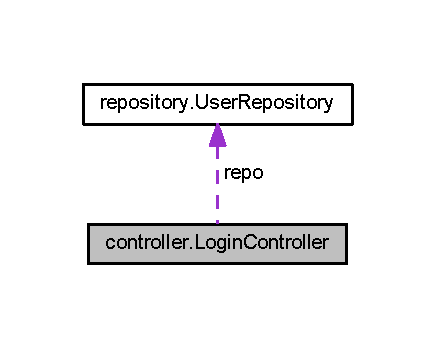
\includegraphics[width=209pt]{classcontroller_1_1_login_controller__coll__graph}
\end{center}
\end{figure}
\subsection*{Public Member Functions}
\begin{DoxyCompactItemize}
\item 
String \mbox{\hyperlink{classcontroller_1_1_login_controller_a98e670c0e2a6a391f1b5b9cb451aedeb}{login}} (Model m, Http\+Servlet\+Response response, Http\+Servlet\+Request request, Web\+Request wrequest)  throws Exception 
\end{DoxyCompactItemize}


\subsection{Detailed Description}
Login class.

\begin{DoxyAuthor}{Author}
Leire 
\end{DoxyAuthor}


\subsection{Member Function Documentation}
\mbox{\Hypertarget{classcontroller_1_1_login_controller_a98e670c0e2a6a391f1b5b9cb451aedeb}\label{classcontroller_1_1_login_controller_a98e670c0e2a6a391f1b5b9cb451aedeb}} 
\index{controller\+::\+Login\+Controller@{controller\+::\+Login\+Controller}!login@{login}}
\index{login@{login}!controller\+::\+Login\+Controller@{controller\+::\+Login\+Controller}}
\subsubsection{\texorpdfstring{login()}{login()}}
{\footnotesize\ttfamily String controller.\+Login\+Controller.\+login (\begin{DoxyParamCaption}\item[{Model}]{m,  }\item[{Http\+Servlet\+Response}]{response,  }\item[{Http\+Servlet\+Request}]{request,  }\item[{Web\+Request}]{wrequest }\end{DoxyParamCaption}) throws Exception\hspace{0.3cm}{\ttfamily [inline]}}

This method will login or register a user and redirect them depending on their type 
\begin{DoxyExceptions}{Exceptions}
{\em Exception} & \\
\hline
\end{DoxyExceptions}


The documentation for this class was generated from the following file\+:\begin{DoxyCompactItemize}
\item 
src/main/java/controller/Login\+Controller.\+java\end{DoxyCompactItemize}

\hypertarget{classcontroller_1_1_manager_controller}{}\section{controller.\+Manager\+Controller Class Reference}
\label{classcontroller_1_1_manager_controller}\index{controller.\+Manager\+Controller@{controller.\+Manager\+Controller}}


Collaboration diagram for controller.\+Manager\+Controller\+:
% FIG 0
\subsection*{Public Member Functions}
\begin{DoxyCompactItemize}
\item 
String \mbox{\hyperlink{classcontroller_1_1_manager_controller_aa49d493a4fb9aa5f0e99f942b21d3991}{customer}} (Model m, Web\+Request request, Http\+Servlet\+Response response, Http\+Servlet\+Request hrequest)  throws I\+O\+Exception 
\item 
String \mbox{\hyperlink{classcontroller_1_1_manager_controller_a59689dd37c44b3294edc931668e57fb0}{orders}} (Model m, Web\+Request request, Http\+Servlet\+Request hrequest, Http\+Servlet\+Response response)  throws I\+O\+Exception 
\item 
String \mbox{\hyperlink{classcontroller_1_1_manager_controller_a32dde55b16d1fb8e38f0a4f1cc0351be}{order}} (Model m, Web\+Request request, Http\+Servlet\+Request hrequest)
\item 
String \mbox{\hyperlink{classcontroller_1_1_manager_controller_a06fcd2a1ad144e711de97430841a804f}{history}} (Model m, Web\+Request request)
\end{DoxyCompactItemize}


\subsection{Detailed Description}
\mbox{\hyperlink{classcontroller_1_1_manager_controller}{Manager\+Controller}} contains the U\+RL actions of the Manager user type \begin{DoxyAuthor}{Author}
Leire 
\end{DoxyAuthor}


\subsection{Member Function Documentation}
\mbox{\Hypertarget{classcontroller_1_1_manager_controller_aa49d493a4fb9aa5f0e99f942b21d3991}\label{classcontroller_1_1_manager_controller_aa49d493a4fb9aa5f0e99f942b21d3991}} 
\index{controller\+::\+Manager\+Controller@{controller\+::\+Manager\+Controller}!customer@{customer}}
\index{customer@{customer}!controller\+::\+Manager\+Controller@{controller\+::\+Manager\+Controller}}
\subsubsection{\texorpdfstring{customer()}{customer()}}
{\footnotesize\ttfamily String controller.\+Manager\+Controller.\+customer (\begin{DoxyParamCaption}\item[{Model}]{m,  }\item[{Web\+Request}]{request,  }\item[{Http\+Servlet\+Response}]{response,  }\item[{Http\+Servlet\+Request}]{hrequest }\end{DoxyParamCaption}) throws I\+O\+Exception\hspace{0.3cm}{\ttfamily [inline]}}

This method will access the manager\textquotesingle{}s main site. 
\begin{DoxyExceptions}{Exceptions}
{\em I\+O\+Exception} & \\
\hline
\end{DoxyExceptions}
\mbox{\Hypertarget{classcontroller_1_1_manager_controller_a06fcd2a1ad144e711de97430841a804f}\label{classcontroller_1_1_manager_controller_a06fcd2a1ad144e711de97430841a804f}} 
\index{controller\+::\+Manager\+Controller@{controller\+::\+Manager\+Controller}!history@{history}}
\index{history@{history}!controller\+::\+Manager\+Controller@{controller\+::\+Manager\+Controller}}
\subsubsection{\texorpdfstring{history()}{history()}}
{\footnotesize\ttfamily String controller.\+Manager\+Controller.\+history (\begin{DoxyParamCaption}\item[{Model}]{m,  }\item[{Web\+Request}]{request }\end{DoxyParamCaption})\hspace{0.3cm}{\ttfamily [inline]}}

This method will access the customer\textquotesingle{}s \textquotesingle{}orders\textquotesingle{} option, where the customer will be able to see the orders made through their history. \mbox{\Hypertarget{classcontroller_1_1_manager_controller_a32dde55b16d1fb8e38f0a4f1cc0351be}\label{classcontroller_1_1_manager_controller_a32dde55b16d1fb8e38f0a4f1cc0351be}} 
\index{controller\+::\+Manager\+Controller@{controller\+::\+Manager\+Controller}!order@{order}}
\index{order@{order}!controller\+::\+Manager\+Controller@{controller\+::\+Manager\+Controller}}
\subsubsection{\texorpdfstring{order()}{order()}}
{\footnotesize\ttfamily String controller.\+Manager\+Controller.\+order (\begin{DoxyParamCaption}\item[{Model}]{m,  }\item[{Web\+Request}]{request,  }\item[{Http\+Servlet\+Request}]{hrequest }\end{DoxyParamCaption})\hspace{0.3cm}{\ttfamily [inline]}}

This method will show an \mbox{\Hypertarget{classcontroller_1_1_manager_controller_a59689dd37c44b3294edc931668e57fb0}\label{classcontroller_1_1_manager_controller_a59689dd37c44b3294edc931668e57fb0}} 
\index{controller\+::\+Manager\+Controller@{controller\+::\+Manager\+Controller}!orders@{orders}}
\index{orders@{orders}!controller\+::\+Manager\+Controller@{controller\+::\+Manager\+Controller}}
\subsubsection{\texorpdfstring{orders()}{orders()}}
{\footnotesize\ttfamily String controller.\+Manager\+Controller.\+orders (\begin{DoxyParamCaption}\item[{Model}]{m,  }\item[{Web\+Request}]{request,  }\item[{Http\+Servlet\+Request}]{hrequest,  }\item[{Http\+Servlet\+Response}]{response }\end{DoxyParamCaption}) throws I\+O\+Exception\hspace{0.3cm}{\ttfamily [inline]}}

This method will access the manager\textquotesingle{}s \textquotesingle{}orders\textquotesingle{} option, where the customer will be able to see the orders made through their history. 
\begin{DoxyExceptions}{Exceptions}
{\em I\+O\+Exception} & \\
\hline
\end{DoxyExceptions}


The documentation for this class was generated from the following file\+:\begin{DoxyCompactItemize}
\item 
D\+:/\+Users/user/\+Documents/\+M\+O\+N\+D\+R\+A/3.\+M\+A\+I\+L\+A/\+P\+O\+P\+B\+L5/\+G\+I\+T/e\+Jkiva\+\_\+\+P\+O\+P\+B\+L5/e\+Jkiva/src/main/java/controller/Manager\+Controller.\+java\end{DoxyCompactItemize}

\hypertarget{classrepository_1_1_manager_repository}{}\section{repository.\+Manager\+Repository Class Reference}
\label{classrepository_1_1_manager_repository}\index{repository.\+Manager\+Repository@{repository.\+Manager\+Repository}}
\subsection*{Public Member Functions}
\begin{DoxyCompactItemize}
\item 
String \mbox{\hyperlink{classrepository_1_1_manager_repository_ae52c653f3008bfa5bc0f5af8dab9db43}{get\+Month}} (int month)
\item 
int \mbox{\hyperlink{classrepository_1_1_manager_repository_a0e915572c7802a1e4503c558cabab270}{get\+Items\+Out\+Value}} (int day, int month)
\item 
Date \mbox{\hyperlink{classrepository_1_1_manager_repository_a674b19911835ed9b14bc4e8ad6bbad95}{get\+Items\+Out\+Date}} (int day, int month)
\item 
\mbox{\hyperlink{classentity_1_1_order}{Order}} \mbox{[}$\,$\mbox{]} \mbox{\hyperlink{classrepository_1_1_manager_repository_aa79e0ef0402a40bb0cc00694ca02adf2}{get\+All\+Orders}} ()
\end{DoxyCompactItemize}


\subsection{Detailed Description}
Manager Repository. Contains functions and sql queries to get information from database used by the customer.

\begin{DoxyAuthor}{Author}
Leire 
\end{DoxyAuthor}


\subsection{Member Function Documentation}
\mbox{\Hypertarget{classrepository_1_1_manager_repository_aa79e0ef0402a40bb0cc00694ca02adf2}\label{classrepository_1_1_manager_repository_aa79e0ef0402a40bb0cc00694ca02adf2}} 
\index{repository\+::\+Manager\+Repository@{repository\+::\+Manager\+Repository}!get\+All\+Orders@{get\+All\+Orders}}
\index{get\+All\+Orders@{get\+All\+Orders}!repository\+::\+Manager\+Repository@{repository\+::\+Manager\+Repository}}
\subsubsection{\texorpdfstring{get\+All\+Orders()}{getAllOrders()}}
{\footnotesize\ttfamily \mbox{\hyperlink{classentity_1_1_order}{Order}} \mbox{[}$\,$\mbox{]} repository.\+Manager\+Repository.\+get\+All\+Orders (\begin{DoxyParamCaption}{ }\end{DoxyParamCaption})\hspace{0.3cm}{\ttfamily [inline]}}

This method will return all the orders of the warehouse\textquotesingle{}s history \begin{DoxyReturn}{Returns}
Order\mbox{[}\mbox{]} 
\end{DoxyReturn}
\mbox{\Hypertarget{classrepository_1_1_manager_repository_a674b19911835ed9b14bc4e8ad6bbad95}\label{classrepository_1_1_manager_repository_a674b19911835ed9b14bc4e8ad6bbad95}} 
\index{repository\+::\+Manager\+Repository@{repository\+::\+Manager\+Repository}!get\+Items\+Out\+Date@{get\+Items\+Out\+Date}}
\index{get\+Items\+Out\+Date@{get\+Items\+Out\+Date}!repository\+::\+Manager\+Repository@{repository\+::\+Manager\+Repository}}
\subsubsection{\texorpdfstring{get\+Items\+Out\+Date()}{getItemsOutDate()}}
{\footnotesize\ttfamily Date repository.\+Manager\+Repository.\+get\+Items\+Out\+Date (\begin{DoxyParamCaption}\item[{int}]{day,  }\item[{int}]{month }\end{DoxyParamCaption})\hspace{0.3cm}{\ttfamily [inline]}}

Function that returns information for the Manager\textquotesingle{}s chart. 
\begin{DoxyParams}{Parameters}
{\em day} & \\
\hline
{\em month} & \\
\hline
\end{DoxyParams}
\begin{DoxyReturn}{Returns}
Date 
\end{DoxyReturn}
\mbox{\Hypertarget{classrepository_1_1_manager_repository_a0e915572c7802a1e4503c558cabab270}\label{classrepository_1_1_manager_repository_a0e915572c7802a1e4503c558cabab270}} 
\index{repository\+::\+Manager\+Repository@{repository\+::\+Manager\+Repository}!get\+Items\+Out\+Value@{get\+Items\+Out\+Value}}
\index{get\+Items\+Out\+Value@{get\+Items\+Out\+Value}!repository\+::\+Manager\+Repository@{repository\+::\+Manager\+Repository}}
\subsubsection{\texorpdfstring{get\+Items\+Out\+Value()}{getItemsOutValue()}}
{\footnotesize\ttfamily int repository.\+Manager\+Repository.\+get\+Items\+Out\+Value (\begin{DoxyParamCaption}\item[{int}]{day,  }\item[{int}]{month }\end{DoxyParamCaption})\hspace{0.3cm}{\ttfamily [inline]}}

Function that returns information for the Manager\textquotesingle{}s chart. 
\begin{DoxyParams}{Parameters}
{\em day} & \\
\hline
{\em month} & \\
\hline
\end{DoxyParams}
\begin{DoxyReturn}{Returns}
int 
\end{DoxyReturn}
\mbox{\Hypertarget{classrepository_1_1_manager_repository_ae52c653f3008bfa5bc0f5af8dab9db43}\label{classrepository_1_1_manager_repository_ae52c653f3008bfa5bc0f5af8dab9db43}} 
\index{repository\+::\+Manager\+Repository@{repository\+::\+Manager\+Repository}!get\+Month@{get\+Month}}
\index{get\+Month@{get\+Month}!repository\+::\+Manager\+Repository@{repository\+::\+Manager\+Repository}}
\subsubsection{\texorpdfstring{get\+Month()}{getMonth()}}
{\footnotesize\ttfamily String repository.\+Manager\+Repository.\+get\+Month (\begin{DoxyParamCaption}\item[{int}]{month }\end{DoxyParamCaption})\hspace{0.3cm}{\ttfamily [inline]}}

Function with a list of Months. 
\begin{DoxyParams}{Parameters}
{\em month} & \\
\hline
\end{DoxyParams}
\begin{DoxyReturn}{Returns}
String 
\end{DoxyReturn}


The documentation for this class was generated from the following file\+:\begin{DoxyCompactItemize}
\item 
src/main/java/repository/Manager\+Repository.\+java\end{DoxyCompactItemize}

\hypertarget{classcontroller_1_1_operator_controller}{}\section{controller.\+Operator\+Controller Class Reference}
\label{classcontroller_1_1_operator_controller}\index{controller.\+Operator\+Controller@{controller.\+Operator\+Controller}}


Collaboration diagram for controller.\+Operator\+Controller\+:
% FIG 0
\subsection*{Public Member Functions}
\begin{DoxyCompactItemize}
\item 
String \mbox{\hyperlink{classcontroller_1_1_operator_controller_af4c2983ca84d7115743de160da84135c}{customer}} (Model m, Web\+Request request, Http\+Servlet\+Response response, Http\+Servlet\+Request hrequest)  throws I\+O\+Exception 
\item 
String \mbox{\hyperlink{classcontroller_1_1_operator_controller_a79b22da6d85dc475cd7973d4f9a47fc1}{orders}} (Model m, Web\+Request request, Http\+Servlet\+Response response, Http\+Servlet\+Request hrequest)  throws I\+O\+Exception 
\item 
String \mbox{\hyperlink{classcontroller_1_1_operator_controller_a1fcb7b5bea154a09eef4db21632bcc60}{order}} (Model m, Web\+Request request, Http\+Servlet\+Response response, Http\+Servlet\+Request hrequest)  throws I\+O\+Exception 
\item 
String \mbox{\hyperlink{classcontroller_1_1_operator_controller_a20f145b080521609c4513dc5544612a2}{stock}} (Model m, Web\+Request request, Http\+Servlet\+Response response, Http\+Servlet\+Request hrequest)  throws I\+O\+Exception 
\end{DoxyCompactItemize}


\subsection{Detailed Description}
\mbox{\hyperlink{classcontroller_1_1_operator_controller}{Operator\+Controller}} contains the U\+RL actions of the Operator user type \begin{DoxyAuthor}{Author}
Leire 
\end{DoxyAuthor}


\subsection{Member Function Documentation}
\mbox{\Hypertarget{classcontroller_1_1_operator_controller_af4c2983ca84d7115743de160da84135c}\label{classcontroller_1_1_operator_controller_af4c2983ca84d7115743de160da84135c}} 
\index{controller\+::\+Operator\+Controller@{controller\+::\+Operator\+Controller}!customer@{customer}}
\index{customer@{customer}!controller\+::\+Operator\+Controller@{controller\+::\+Operator\+Controller}}
\subsubsection{\texorpdfstring{customer()}{customer()}}
{\footnotesize\ttfamily String controller.\+Operator\+Controller.\+customer (\begin{DoxyParamCaption}\item[{Model}]{m,  }\item[{Web\+Request}]{request,  }\item[{Http\+Servlet\+Response}]{response,  }\item[{Http\+Servlet\+Request}]{hrequest }\end{DoxyParamCaption}) throws I\+O\+Exception\hspace{0.3cm}{\ttfamily [inline]}}

This method will access the operator\textquotesingle{}s main site. 
\begin{DoxyExceptions}{Exceptions}
{\em I\+O\+Exception} & \\
\hline
\end{DoxyExceptions}
\mbox{\Hypertarget{classcontroller_1_1_operator_controller_a1fcb7b5bea154a09eef4db21632bcc60}\label{classcontroller_1_1_operator_controller_a1fcb7b5bea154a09eef4db21632bcc60}} 
\index{controller\+::\+Operator\+Controller@{controller\+::\+Operator\+Controller}!order@{order}}
\index{order@{order}!controller\+::\+Operator\+Controller@{controller\+::\+Operator\+Controller}}
\subsubsection{\texorpdfstring{order()}{order()}}
{\footnotesize\ttfamily String controller.\+Operator\+Controller.\+order (\begin{DoxyParamCaption}\item[{Model}]{m,  }\item[{Web\+Request}]{request,  }\item[{Http\+Servlet\+Response}]{response,  }\item[{Http\+Servlet\+Request}]{hrequest }\end{DoxyParamCaption}) throws I\+O\+Exception\hspace{0.3cm}{\ttfamily [inline]}}

This method will access the customer\textquotesingle{}s \textquotesingle{}orders\textquotesingle{} option, where the customer will be able to see the orders made through their history. 
\begin{DoxyExceptions}{Exceptions}
{\em I\+O\+Exception} & \\
\hline
\end{DoxyExceptions}
\mbox{\Hypertarget{classcontroller_1_1_operator_controller_a79b22da6d85dc475cd7973d4f9a47fc1}\label{classcontroller_1_1_operator_controller_a79b22da6d85dc475cd7973d4f9a47fc1}} 
\index{controller\+::\+Operator\+Controller@{controller\+::\+Operator\+Controller}!orders@{orders}}
\index{orders@{orders}!controller\+::\+Operator\+Controller@{controller\+::\+Operator\+Controller}}
\subsubsection{\texorpdfstring{orders()}{orders()}}
{\footnotesize\ttfamily String controller.\+Operator\+Controller.\+orders (\begin{DoxyParamCaption}\item[{Model}]{m,  }\item[{Web\+Request}]{request,  }\item[{Http\+Servlet\+Response}]{response,  }\item[{Http\+Servlet\+Request}]{hrequest }\end{DoxyParamCaption}) throws I\+O\+Exception\hspace{0.3cm}{\ttfamily [inline]}}

This method will access the customer\textquotesingle{}s \textquotesingle{}orders\textquotesingle{} option, where the customer will be able to see the orders made through their history. 
\begin{DoxyExceptions}{Exceptions}
{\em I\+O\+Exception} & \\
\hline
\end{DoxyExceptions}
\mbox{\Hypertarget{classcontroller_1_1_operator_controller_a20f145b080521609c4513dc5544612a2}\label{classcontroller_1_1_operator_controller_a20f145b080521609c4513dc5544612a2}} 
\index{controller\+::\+Operator\+Controller@{controller\+::\+Operator\+Controller}!stock@{stock}}
\index{stock@{stock}!controller\+::\+Operator\+Controller@{controller\+::\+Operator\+Controller}}
\subsubsection{\texorpdfstring{stock()}{stock()}}
{\footnotesize\ttfamily String controller.\+Operator\+Controller.\+stock (\begin{DoxyParamCaption}\item[{Model}]{m,  }\item[{Web\+Request}]{request,  }\item[{Http\+Servlet\+Response}]{response,  }\item[{Http\+Servlet\+Request}]{hrequest }\end{DoxyParamCaption}) throws I\+O\+Exception\hspace{0.3cm}{\ttfamily [inline]}}

This method will access the customer\textquotesingle{}s \textquotesingle{}orders\textquotesingle{} option, where the customer will be able to see the orders made through their history. 
\begin{DoxyExceptions}{Exceptions}
{\em I\+O\+Exception} & \\
\hline
\end{DoxyExceptions}


The documentation for this class was generated from the following file\+:\begin{DoxyCompactItemize}
\item 
D\+:/\+Users/user/\+Documents/\+M\+O\+N\+D\+R\+A/3.\+M\+A\+I\+L\+A/\+P\+O\+P\+B\+L5/\+G\+I\+T/e\+Jkiva\+\_\+\+P\+O\+P\+B\+L5/e\+Jkiva/src/main/java/controller/Operator\+Controller.\+java\end{DoxyCompactItemize}

\hypertarget{classrepository_1_1_operator_repository}{}\section{repository.\+Operator\+Repository Class Reference}
\label{classrepository_1_1_operator_repository}\index{repository.\+Operator\+Repository@{repository.\+Operator\+Repository}}
\subsection*{Public Member Functions}
\begin{DoxyCompactItemize}
\item 
\mbox{\hyperlink{classentity_1_1_order}{Order}} \mbox{[}$\,$\mbox{]} \mbox{\hyperlink{classrepository_1_1_operator_repository_ac371d50c4b824da2d066da12be265aef}{get\+All\+Orders}} ()
\end{DoxyCompactItemize}


\subsection{Member Function Documentation}
\mbox{\Hypertarget{classrepository_1_1_operator_repository_ac371d50c4b824da2d066da12be265aef}\label{classrepository_1_1_operator_repository_ac371d50c4b824da2d066da12be265aef}} 
\index{repository\+::\+Operator\+Repository@{repository\+::\+Operator\+Repository}!get\+All\+Orders@{get\+All\+Orders}}
\index{get\+All\+Orders@{get\+All\+Orders}!repository\+::\+Operator\+Repository@{repository\+::\+Operator\+Repository}}
\subsubsection{\texorpdfstring{get\+All\+Orders()}{getAllOrders()}}
{\footnotesize\ttfamily \mbox{\hyperlink{classentity_1_1_order}{Order}} \mbox{[}$\,$\mbox{]} repository.\+Operator\+Repository.\+get\+All\+Orders (\begin{DoxyParamCaption}{ }\end{DoxyParamCaption})\hspace{0.3cm}{\ttfamily [inline]}}

This method will return all the orders of the user given 

The documentation for this class was generated from the following file\+:\begin{DoxyCompactItemize}
\item 
D\+:/\+Users/user/\+Documents/\+M\+O\+N\+D\+R\+A/3.\+M\+A\+I\+L\+A/\+P\+O\+P\+B\+L5/\+G\+I\+T/e\+Jkiva\+\_\+\+P\+O\+P\+B\+L5/e\+Jkiva/src/main/java/repository/Operator\+Repository.\+java\end{DoxyCompactItemize}

\hypertarget{classentity_1_1_order}{}\section{entity.\+Order Class Reference}
\label{classentity_1_1_order}\index{entity.\+Order@{entity.\+Order}}


Inheritance diagram for entity.\+Order\+:\nopagebreak
\begin{figure}[H]
\begin{center}
\leavevmode
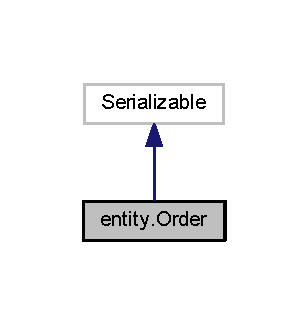
\includegraphics[width=148pt]{classentity_1_1_order__inherit__graph}
\end{center}
\end{figure}


Collaboration diagram for entity.\+Order\+:\nopagebreak
\begin{figure}[H]
\begin{center}
\leavevmode
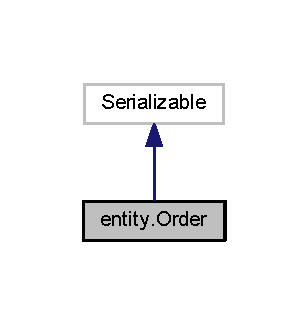
\includegraphics[width=148pt]{classentity_1_1_order__coll__graph}
\end{center}
\end{figure}
\subsection*{Public Member Functions}
\begin{DoxyCompactItemize}
\item 
\mbox{\Hypertarget{classentity_1_1_order_a29eb9dead0b1577bd57bc3a5db15f981}\label{classentity_1_1_order_a29eb9dead0b1577bd57bc3a5db15f981}} 
{\bfseries Order} (\mbox{\hyperlink{classentity_1_1_user}{User}} user, Date date\+Order)
\item 
\mbox{\Hypertarget{classentity_1_1_order_a5180af95fecce83f0416706550fed72d}\label{classentity_1_1_order_a5180af95fecce83f0416706550fed72d}} 
{\bfseries Order} (\mbox{\hyperlink{classentity_1_1_user}{User}} user, Date date\+Order, Date date\+Delivered)
\item 
\mbox{\Hypertarget{classentity_1_1_order_a4561af92f26502434e496c32164ea1ff}\label{classentity_1_1_order_a4561af92f26502434e496c32164ea1ff}} 
int {\bfseries get\+Order\+Id} ()
\item 
\mbox{\Hypertarget{classentity_1_1_order_a780f89a2c6102d22cc7c076b7a038c8f}\label{classentity_1_1_order_a780f89a2c6102d22cc7c076b7a038c8f}} 
void {\bfseries set\+Order\+Id} (int order\+Id)
\item 
\mbox{\Hypertarget{classentity_1_1_order_a5262114e6d86f0826384b5aebaa04856}\label{classentity_1_1_order_a5262114e6d86f0826384b5aebaa04856}} 
\mbox{\hyperlink{classentity_1_1_user}{User}} {\bfseries get\+User} ()
\item 
\mbox{\Hypertarget{classentity_1_1_order_ad8de4f52695d2a9230e9bdb0aa42decb}\label{classentity_1_1_order_ad8de4f52695d2a9230e9bdb0aa42decb}} 
void {\bfseries set\+User} (\mbox{\hyperlink{classentity_1_1_user}{User}} user)
\item 
\mbox{\Hypertarget{classentity_1_1_order_a69a26d54af50e17b399f6af80433b569}\label{classentity_1_1_order_a69a26d54af50e17b399f6af80433b569}} 
Date {\bfseries get\+Date\+Order} ()
\item 
\mbox{\Hypertarget{classentity_1_1_order_a0c2fee67a9b341a27e83b875534bf9ea}\label{classentity_1_1_order_a0c2fee67a9b341a27e83b875534bf9ea}} 
void {\bfseries set\+Date\+Order} (Date date\+Order)
\item 
\mbox{\Hypertarget{classentity_1_1_order_a949fad3af9e1747db36124d934ed6413}\label{classentity_1_1_order_a949fad3af9e1747db36124d934ed6413}} 
Date {\bfseries get\+Date\+Delivered} ()
\item 
\mbox{\Hypertarget{classentity_1_1_order_a36942ca27b3ac8f905319ba13986ff19}\label{classentity_1_1_order_a36942ca27b3ac8f905319ba13986ff19}} 
void {\bfseries set\+Date\+Delivered} (Date date\+Delivered)
\end{DoxyCompactItemize}


\subsection{Detailed Description}
\mbox{\hyperlink{classentity_1_1_order}{Order}} generated by hbm2java 

The documentation for this class was generated from the following file\+:\begin{DoxyCompactItemize}
\item 
src/main/java/entity/Order.\+java\end{DoxyCompactItemize}

\hypertarget{classentity_1_1copy_1_1_order}{}\section{entity.\+copy.\+Order Class Reference}
\label{classentity_1_1copy_1_1_order}\index{entity.\+copy.\+Order@{entity.\+copy.\+Order}}


Inheritance diagram for entity.\+copy.\+Order\+:
% FIG 0


Collaboration diagram for entity.\+copy.\+Order\+:
% FIG 1
\subsection*{Public Member Functions}
\begin{DoxyCompactItemize}
\item 
\mbox{\Hypertarget{classentity_1_1copy_1_1_order_aee666f6da3c8bb8cfe4ce3699aa7fce2}\label{classentity_1_1copy_1_1_order_aee666f6da3c8bb8cfe4ce3699aa7fce2}} 
{\bfseries Order} (\mbox{\hyperlink{classentity_1_1copy_1_1_user}{User}} user, Date date)
\item 
\mbox{\Hypertarget{classentity_1_1copy_1_1_order_af2ac4a03d75f6dce4f224a1728dab6f0}\label{classentity_1_1copy_1_1_order_af2ac4a03d75f6dce4f224a1728dab6f0}} 
int {\bfseries get\+Order\+Id} ()
\item 
\mbox{\Hypertarget{classentity_1_1copy_1_1_order_ad9a5ee04f79b8c74569a76d529122e4f}\label{classentity_1_1copy_1_1_order_ad9a5ee04f79b8c74569a76d529122e4f}} 
void {\bfseries set\+Order\+Id} (int order\+Id)
\item 
\mbox{\Hypertarget{classentity_1_1copy_1_1_order_ab47f88a27fae5d395ef0d5464b686e65}\label{classentity_1_1copy_1_1_order_ab47f88a27fae5d395ef0d5464b686e65}} 
\mbox{\hyperlink{classentity_1_1copy_1_1_user}{User}} {\bfseries get\+User} ()
\item 
\mbox{\Hypertarget{classentity_1_1copy_1_1_order_a7820d3309c881e54099ea477ea1dd4cf}\label{classentity_1_1copy_1_1_order_a7820d3309c881e54099ea477ea1dd4cf}} 
void {\bfseries set\+User} (\mbox{\hyperlink{classentity_1_1copy_1_1_user}{User}} user)
\item 
\mbox{\Hypertarget{classentity_1_1copy_1_1_order_a0c3568ec65e20efd5357ecdb37899d01}\label{classentity_1_1copy_1_1_order_a0c3568ec65e20efd5357ecdb37899d01}} 
Date {\bfseries get\+Date} ()
\item 
\mbox{\Hypertarget{classentity_1_1copy_1_1_order_a91aa08696dcbde232e8f700ee1371dd3}\label{classentity_1_1copy_1_1_order_a91aa08696dcbde232e8f700ee1371dd3}} 
void {\bfseries set\+Date} (Date date)
\end{DoxyCompactItemize}


\subsection{Detailed Description}
\mbox{\hyperlink{classentity_1_1copy_1_1_order}{Order}} generated by hbm2java 

The documentation for this class was generated from the following file\+:\begin{DoxyCompactItemize}
\item 
D\+:/\+Users/user/\+Documents/\+M\+O\+N\+D\+R\+A/3.\+M\+A\+I\+L\+A/\+P\+O\+P\+B\+L5/\+G\+I\+T/e\+Jkiva\+\_\+\+P\+O\+P\+B\+L5/e\+Jkiva/src/main/java/entity/copy/Order.\+java\end{DoxyCompactItemize}

\hypertarget{classentity_1_1_orderproduct}{}\section{entity.\+Orderproduct Class Reference}
\label{classentity_1_1_orderproduct}\index{entity.\+Orderproduct@{entity.\+Orderproduct}}


Inheritance diagram for entity.\+Orderproduct\+:
% FIG 0


Collaboration diagram for entity.\+Orderproduct\+:
% FIG 1
\subsection*{Public Member Functions}
\begin{DoxyCompactItemize}
\item 
\mbox{\Hypertarget{classentity_1_1_orderproduct_a141723329278c6424a1d300db29529a4}\label{classentity_1_1_orderproduct_a141723329278c6424a1d300db29529a4}} 
{\bfseries Orderproduct} (\mbox{\hyperlink{classentity_1_1_order}{Order}} order, \mbox{\hyperlink{classentity_1_1_product}{Product}} product, short quantity)
\item 
\mbox{\Hypertarget{classentity_1_1_orderproduct_a08d3bfc82478033cba0386026800358b}\label{classentity_1_1_orderproduct_a08d3bfc82478033cba0386026800358b}} 
int {\bfseries get\+Order\+Product\+Id} ()
\item 
\mbox{\Hypertarget{classentity_1_1_orderproduct_afb5336d8fb886081876eb8b69970daad}\label{classentity_1_1_orderproduct_afb5336d8fb886081876eb8b69970daad}} 
void {\bfseries set\+Order\+Product\+Id} (int order\+Product\+Id)
\item 
\mbox{\Hypertarget{classentity_1_1_orderproduct_af160d989a7a8c448ce983743a8ee1578}\label{classentity_1_1_orderproduct_af160d989a7a8c448ce983743a8ee1578}} 
\mbox{\hyperlink{classentity_1_1_order}{Order}} {\bfseries get\+Order} ()
\item 
\mbox{\Hypertarget{classentity_1_1_orderproduct_ac38152f038c0669a8f2280c6f55fc1bb}\label{classentity_1_1_orderproduct_ac38152f038c0669a8f2280c6f55fc1bb}} 
void {\bfseries set\+Order} (\mbox{\hyperlink{classentity_1_1_order}{Order}} order)
\item 
\mbox{\Hypertarget{classentity_1_1_orderproduct_ac8a5d534f8433a8260ea87a85bb00217}\label{classentity_1_1_orderproduct_ac8a5d534f8433a8260ea87a85bb00217}} 
\mbox{\hyperlink{classentity_1_1_product}{Product}} {\bfseries get\+Product} ()
\item 
\mbox{\Hypertarget{classentity_1_1_orderproduct_a4d9fd082a96c982443e6ad4cfb032a61}\label{classentity_1_1_orderproduct_a4d9fd082a96c982443e6ad4cfb032a61}} 
void {\bfseries set\+Product} (\mbox{\hyperlink{classentity_1_1_product}{Product}} product)
\item 
\mbox{\Hypertarget{classentity_1_1_orderproduct_a4a10cb8ecd7ac4c692f5f3fa96793e9d}\label{classentity_1_1_orderproduct_a4a10cb8ecd7ac4c692f5f3fa96793e9d}} 
short {\bfseries get\+Quantity} ()
\item 
\mbox{\Hypertarget{classentity_1_1_orderproduct_ab402591f6605ff9ad60a62175b4e6d0d}\label{classentity_1_1_orderproduct_ab402591f6605ff9ad60a62175b4e6d0d}} 
void {\bfseries set\+Quantity} (short quantity)
\end{DoxyCompactItemize}


\subsection{Detailed Description}
\mbox{\hyperlink{classentity_1_1_orderproduct}{Orderproduct}} generated by hbm2java 

The documentation for this class was generated from the following file\+:\begin{DoxyCompactItemize}
\item 
D\+:/\+Users/user/\+Documents/\+M\+O\+N\+D\+R\+A/3.\+M\+A\+I\+L\+A/\+P\+O\+P\+B\+L5/\+G\+I\+T/e\+Jkiva\+\_\+\+P\+O\+P\+B\+L5/e\+Jkiva/src/main/java/entity/Orderproduct.\+java\end{DoxyCompactItemize}

\hypertarget{classentity_1_1copy_1_1_orderproduct}{}\section{entity.\+copy.\+Orderproduct Class Reference}
\label{classentity_1_1copy_1_1_orderproduct}\index{entity.\+copy.\+Orderproduct@{entity.\+copy.\+Orderproduct}}


Inheritance diagram for entity.\+copy.\+Orderproduct\+:
% FIG 0


Collaboration diagram for entity.\+copy.\+Orderproduct\+:
% FIG 1
\subsection*{Public Member Functions}
\begin{DoxyCompactItemize}
\item 
\mbox{\Hypertarget{classentity_1_1copy_1_1_orderproduct_ab7f6fed29d1697ec8d704002338fd840}\label{classentity_1_1copy_1_1_orderproduct_ab7f6fed29d1697ec8d704002338fd840}} 
{\bfseries Orderproduct} (\mbox{\hyperlink{classentity_1_1copy_1_1_order}{Order}} order, \mbox{\hyperlink{classentity_1_1copy_1_1_product}{Product}} product, short quantity)
\item 
\mbox{\Hypertarget{classentity_1_1copy_1_1_orderproduct_a659a540d9dd34e67dce92c2c8ad1f9c6}\label{classentity_1_1copy_1_1_orderproduct_a659a540d9dd34e67dce92c2c8ad1f9c6}} 
int {\bfseries get\+Order\+Product\+Id} ()
\item 
\mbox{\Hypertarget{classentity_1_1copy_1_1_orderproduct_ad689ca8d2521567a1bf983067d225fd6}\label{classentity_1_1copy_1_1_orderproduct_ad689ca8d2521567a1bf983067d225fd6}} 
void {\bfseries set\+Order\+Product\+Id} (int order\+Product\+Id)
\item 
\mbox{\Hypertarget{classentity_1_1copy_1_1_orderproduct_a6af4a2b7aca0d72695ab12ef2d542004}\label{classentity_1_1copy_1_1_orderproduct_a6af4a2b7aca0d72695ab12ef2d542004}} 
\mbox{\hyperlink{classentity_1_1copy_1_1_order}{Order}} {\bfseries get\+Order} ()
\item 
\mbox{\Hypertarget{classentity_1_1copy_1_1_orderproduct_aea27a0c453a89d2367f411dc7f9c95ba}\label{classentity_1_1copy_1_1_orderproduct_aea27a0c453a89d2367f411dc7f9c95ba}} 
void {\bfseries set\+Order} (\mbox{\hyperlink{classentity_1_1copy_1_1_order}{Order}} order)
\item 
\mbox{\Hypertarget{classentity_1_1copy_1_1_orderproduct_add40f07b41fc7923ae8fe1b36e257deb}\label{classentity_1_1copy_1_1_orderproduct_add40f07b41fc7923ae8fe1b36e257deb}} 
\mbox{\hyperlink{classentity_1_1copy_1_1_product}{Product}} {\bfseries get\+Product} ()
\item 
\mbox{\Hypertarget{classentity_1_1copy_1_1_orderproduct_a919266deed77c0f42824ea923da340af}\label{classentity_1_1copy_1_1_orderproduct_a919266deed77c0f42824ea923da340af}} 
void {\bfseries set\+Product} (\mbox{\hyperlink{classentity_1_1copy_1_1_product}{Product}} product)
\item 
\mbox{\Hypertarget{classentity_1_1copy_1_1_orderproduct_a50c5839107b066502b566dd6a56ebd74}\label{classentity_1_1copy_1_1_orderproduct_a50c5839107b066502b566dd6a56ebd74}} 
short {\bfseries get\+Quantity} ()
\item 
\mbox{\Hypertarget{classentity_1_1copy_1_1_orderproduct_af6b91f509a7bf6c54055d4a56d4723e3}\label{classentity_1_1copy_1_1_orderproduct_af6b91f509a7bf6c54055d4a56d4723e3}} 
void {\bfseries set\+Quantity} (short quantity)
\end{DoxyCompactItemize}


\subsection{Detailed Description}
\mbox{\hyperlink{classentity_1_1copy_1_1_orderproduct}{Orderproduct}} generated by hbm2java 

The documentation for this class was generated from the following file\+:\begin{DoxyCompactItemize}
\item 
D\+:/\+Users/user/\+Documents/\+M\+O\+N\+D\+R\+A/3.\+M\+A\+I\+L\+A/\+P\+O\+P\+B\+L5/\+G\+I\+T/e\+Jkiva\+\_\+\+P\+O\+P\+B\+L5/e\+Jkiva/src/main/java/entity/copy/Orderproduct.\+java\end{DoxyCompactItemize}

\hypertarget{classentity_1_1copy_1_1_product}{}\section{entity.\+copy.\+Product Class Reference}
\label{classentity_1_1copy_1_1_product}\index{entity.\+copy.\+Product@{entity.\+copy.\+Product}}


Inheritance diagram for entity.\+copy.\+Product\+:
% FIG 0


Collaboration diagram for entity.\+copy.\+Product\+:
% FIG 1
\subsection*{Public Member Functions}
\begin{DoxyCompactItemize}
\item 
\mbox{\Hypertarget{classentity_1_1copy_1_1_product_a92a818422328af74cedead5bb76d2312}\label{classentity_1_1copy_1_1_product_a92a818422328af74cedead5bb76d2312}} 
{\bfseries Product} (String product\+Name, float price)
\item 
\mbox{\Hypertarget{classentity_1_1copy_1_1_product_a06b960cea288dbf04e271b8b5d39ccc6}\label{classentity_1_1copy_1_1_product_a06b960cea288dbf04e271b8b5d39ccc6}} 
{\bfseries Product} (\mbox{\hyperlink{classentity_1_1copy_1_1_departament}{Departament}} departament, String product\+Name, String description, float price)
\item 
\mbox{\Hypertarget{classentity_1_1copy_1_1_product_a2f8741b135f534044764953684b6b572}\label{classentity_1_1copy_1_1_product_a2f8741b135f534044764953684b6b572}} 
int {\bfseries get\+Product\+Id} ()
\item 
\mbox{\Hypertarget{classentity_1_1copy_1_1_product_a420f74ca7a14413440a9a8f4d2b0a9d3}\label{classentity_1_1copy_1_1_product_a420f74ca7a14413440a9a8f4d2b0a9d3}} 
void {\bfseries set\+Product\+Id} (int product\+Id)
\item 
\mbox{\Hypertarget{classentity_1_1copy_1_1_product_a4156850c240ef741fbed8fc4644c65ac}\label{classentity_1_1copy_1_1_product_a4156850c240ef741fbed8fc4644c65ac}} 
\mbox{\hyperlink{classentity_1_1copy_1_1_departament}{Departament}} {\bfseries get\+Departament} ()
\item 
\mbox{\Hypertarget{classentity_1_1copy_1_1_product_a64b331b630bfb3b18eb90a8e053b3257}\label{classentity_1_1copy_1_1_product_a64b331b630bfb3b18eb90a8e053b3257}} 
void {\bfseries set\+Departament} (\mbox{\hyperlink{classentity_1_1copy_1_1_departament}{Departament}} departament)
\item 
\mbox{\Hypertarget{classentity_1_1copy_1_1_product_a8644d8829d4254346993bdc7b4c7a8ba}\label{classentity_1_1copy_1_1_product_a8644d8829d4254346993bdc7b4c7a8ba}} 
String {\bfseries get\+Product\+Name} ()
\item 
\mbox{\Hypertarget{classentity_1_1copy_1_1_product_a9a47aa091bbd8d534810fffb1407ccd8}\label{classentity_1_1copy_1_1_product_a9a47aa091bbd8d534810fffb1407ccd8}} 
void {\bfseries set\+Product\+Name} (String product\+Name)
\item 
\mbox{\Hypertarget{classentity_1_1copy_1_1_product_a43b93cfcc32200cb7a1cce47e90117f6}\label{classentity_1_1copy_1_1_product_a43b93cfcc32200cb7a1cce47e90117f6}} 
String {\bfseries get\+Description} ()
\item 
\mbox{\Hypertarget{classentity_1_1copy_1_1_product_a701999a3460085d6e71fcd163a24dc2b}\label{classentity_1_1copy_1_1_product_a701999a3460085d6e71fcd163a24dc2b}} 
void {\bfseries set\+Description} (String description)
\item 
\mbox{\Hypertarget{classentity_1_1copy_1_1_product_aea3fb9d5f363805dd3a437454a437135}\label{classentity_1_1copy_1_1_product_aea3fb9d5f363805dd3a437454a437135}} 
float {\bfseries get\+Price} ()
\item 
\mbox{\Hypertarget{classentity_1_1copy_1_1_product_a7dffc059d4324b75eed57b54a00a2856}\label{classentity_1_1copy_1_1_product_a7dffc059d4324b75eed57b54a00a2856}} 
void {\bfseries set\+Price} (float price)
\item 
\mbox{\Hypertarget{classentity_1_1copy_1_1_product_a346da789eabee1b788186e1170469dd5}\label{classentity_1_1copy_1_1_product_a346da789eabee1b788186e1170469dd5}} 
String {\bfseries to\+String} ()
\end{DoxyCompactItemize}


\subsection{Detailed Description}
\mbox{\hyperlink{classentity_1_1copy_1_1_product}{Product}} generated by hbm2java 

The documentation for this class was generated from the following file\+:\begin{DoxyCompactItemize}
\item 
D\+:/\+Users/user/\+Documents/\+M\+O\+N\+D\+R\+A/3.\+M\+A\+I\+L\+A/\+P\+O\+P\+B\+L5/\+G\+I\+T/e\+Jkiva\+\_\+\+P\+O\+P\+B\+L5/e\+Jkiva/src/main/java/entity/copy/Product.\+java\end{DoxyCompactItemize}

\hypertarget{classentity_1_1_product}{}\section{entity.\+Product Class Reference}
\label{classentity_1_1_product}\index{entity.\+Product@{entity.\+Product}}


Inheritance diagram for entity.\+Product\+:
% FIG 0


Collaboration diagram for entity.\+Product\+:
% FIG 1
\subsection*{Public Member Functions}
\begin{DoxyCompactItemize}
\item 
\mbox{\Hypertarget{classentity_1_1_product_a16490d212d113e14eb833a18ffd35c9e}\label{classentity_1_1_product_a16490d212d113e14eb833a18ffd35c9e}} 
{\bfseries Product} (String product\+Name, float price)
\item 
\mbox{\Hypertarget{classentity_1_1_product_aac8d06cb1b251960fd960abec0ed08ce}\label{classentity_1_1_product_aac8d06cb1b251960fd960abec0ed08ce}} 
{\bfseries Product} (\mbox{\hyperlink{classentity_1_1_departament}{Departament}} departament, String product\+Name, String description, float price, String image)
\item 
\mbox{\Hypertarget{classentity_1_1_product_a2d097a6e21ca5384407ef2d5629409d0}\label{classentity_1_1_product_a2d097a6e21ca5384407ef2d5629409d0}} 
int {\bfseries get\+Product\+Id} ()
\item 
\mbox{\Hypertarget{classentity_1_1_product_ad9a9458cf69f508b1d80cd90f4649343}\label{classentity_1_1_product_ad9a9458cf69f508b1d80cd90f4649343}} 
void {\bfseries set\+Product\+Id} (int product\+Id)
\item 
\mbox{\Hypertarget{classentity_1_1_product_a78bd5ae5f85a3d22bdd23b84c07f1ed4}\label{classentity_1_1_product_a78bd5ae5f85a3d22bdd23b84c07f1ed4}} 
\mbox{\hyperlink{classentity_1_1_departament}{Departament}} {\bfseries get\+Departament} ()
\item 
\mbox{\Hypertarget{classentity_1_1_product_aa67771d630e8eb1922b751a266df6a62}\label{classentity_1_1_product_aa67771d630e8eb1922b751a266df6a62}} 
void {\bfseries set\+Departament} (\mbox{\hyperlink{classentity_1_1_departament}{Departament}} departament)
\item 
\mbox{\Hypertarget{classentity_1_1_product_a81d43916d1f7b73a2f087e3570d73de0}\label{classentity_1_1_product_a81d43916d1f7b73a2f087e3570d73de0}} 
String {\bfseries get\+Product\+Name} ()
\item 
\mbox{\Hypertarget{classentity_1_1_product_abbed2e3b34beb9eff42595b8e2641f7a}\label{classentity_1_1_product_abbed2e3b34beb9eff42595b8e2641f7a}} 
void {\bfseries set\+Product\+Name} (String product\+Name)
\item 
\mbox{\Hypertarget{classentity_1_1_product_a33ba8df9ce2e2cbf6091bb97a0ee0f2c}\label{classentity_1_1_product_a33ba8df9ce2e2cbf6091bb97a0ee0f2c}} 
String {\bfseries get\+Description} ()
\item 
\mbox{\Hypertarget{classentity_1_1_product_a275f824222328131f6a00f383196da41}\label{classentity_1_1_product_a275f824222328131f6a00f383196da41}} 
void {\bfseries set\+Description} (String description)
\item 
\mbox{\Hypertarget{classentity_1_1_product_af6bbc7b34e0ab7b7f2fe758d174fa5f4}\label{classentity_1_1_product_af6bbc7b34e0ab7b7f2fe758d174fa5f4}} 
float {\bfseries get\+Price} ()
\item 
\mbox{\Hypertarget{classentity_1_1_product_a096085200f5ea9730661bc114a0f929d}\label{classentity_1_1_product_a096085200f5ea9730661bc114a0f929d}} 
void {\bfseries set\+Price} (float price)
\item 
\mbox{\Hypertarget{classentity_1_1_product_a5466888d66016874eb475a2703cbc709}\label{classentity_1_1_product_a5466888d66016874eb475a2703cbc709}} 
String {\bfseries get\+Image} ()
\item 
\mbox{\Hypertarget{classentity_1_1_product_a02b293f40f4d82e30617fdc2be6fac49}\label{classentity_1_1_product_a02b293f40f4d82e30617fdc2be6fac49}} 
void {\bfseries set\+Image} (String image)
\item 
\mbox{\Hypertarget{classentity_1_1_product_ad77da4f2b6b67974fd2a040e2b930970}\label{classentity_1_1_product_ad77da4f2b6b67974fd2a040e2b930970}} 
String {\bfseries to\+String} ()
\end{DoxyCompactItemize}


\subsection{Detailed Description}
\mbox{\hyperlink{classentity_1_1_product}{Product}} generated by hbm2java 

The documentation for this class was generated from the following file\+:\begin{DoxyCompactItemize}
\item 
D\+:/\+Users/user/\+Documents/\+M\+O\+N\+D\+R\+A/3.\+M\+A\+I\+L\+A/\+P\+O\+P\+B\+L5/\+G\+I\+T/e\+Jkiva\+\_\+\+P\+O\+P\+B\+L5/e\+Jkiva/src/main/java/entity/Product.\+java\end{DoxyCompactItemize}

\hypertarget{classentity_1_1copy_1_1_segment}{}\section{entity.\+copy.\+Segment Class Reference}
\label{classentity_1_1copy_1_1_segment}\index{entity.\+copy.\+Segment@{entity.\+copy.\+Segment}}


Inheritance diagram for entity.\+copy.\+Segment\+:
% FIG 0


Collaboration diagram for entity.\+copy.\+Segment\+:
% FIG 1
\subsection*{Public Member Functions}
\begin{DoxyCompactItemize}
\item 
\mbox{\Hypertarget{classentity_1_1copy_1_1_segment_a813c6070191056d5a39f14ab8760eb61}\label{classentity_1_1copy_1_1_segment_a813c6070191056d5a39f14ab8760eb61}} 
{\bfseries Segment} (String segment, short posX, short posY)
\item 
\mbox{\Hypertarget{classentity_1_1copy_1_1_segment_ada1f074c6575c766d0cabd2d644fe795}\label{classentity_1_1copy_1_1_segment_ada1f074c6575c766d0cabd2d644fe795}} 
{\bfseries Segment} (String segment, short posX, short posY, String description, Set authomaches, Set workstations)
\item 
\mbox{\Hypertarget{classentity_1_1copy_1_1_segment_a7e8b1178e3f03b902bbb8ebc071ab2b0}\label{classentity_1_1copy_1_1_segment_a7e8b1178e3f03b902bbb8ebc071ab2b0}} 
int {\bfseries get\+Segment\+Id} ()
\item 
\mbox{\Hypertarget{classentity_1_1copy_1_1_segment_a97b528d127b770d7d7b8afad141eda72}\label{classentity_1_1copy_1_1_segment_a97b528d127b770d7d7b8afad141eda72}} 
void {\bfseries set\+Segment\+Id} (Byte segment\+Id)
\item 
\mbox{\Hypertarget{classentity_1_1copy_1_1_segment_ad1ee3e2ff33fc76c72828f050145969b}\label{classentity_1_1copy_1_1_segment_ad1ee3e2ff33fc76c72828f050145969b}} 
String {\bfseries get\+Segment} ()
\item 
\mbox{\Hypertarget{classentity_1_1copy_1_1_segment_a87a1c93a1462201e180e97942e55ff43}\label{classentity_1_1copy_1_1_segment_a87a1c93a1462201e180e97942e55ff43}} 
void {\bfseries set\+Segment} (String segment)
\item 
\mbox{\Hypertarget{classentity_1_1copy_1_1_segment_af3182267c53965e141a9174cd949b859}\label{classentity_1_1copy_1_1_segment_af3182267c53965e141a9174cd949b859}} 
short {\bfseries get\+PosX} ()
\item 
\mbox{\Hypertarget{classentity_1_1copy_1_1_segment_a484a875d3998b86c9e2785dda92c80be}\label{classentity_1_1copy_1_1_segment_a484a875d3998b86c9e2785dda92c80be}} 
void {\bfseries set\+PosX} (short posX)
\item 
\mbox{\Hypertarget{classentity_1_1copy_1_1_segment_afeff5d69389c11594aea4c8022b091aa}\label{classentity_1_1copy_1_1_segment_afeff5d69389c11594aea4c8022b091aa}} 
short {\bfseries get\+PosY} ()
\item 
\mbox{\Hypertarget{classentity_1_1copy_1_1_segment_a723be68a00fd5ba6b611ae1a422623db}\label{classentity_1_1copy_1_1_segment_a723be68a00fd5ba6b611ae1a422623db}} 
void {\bfseries set\+PosY} (short posY)
\item 
\mbox{\Hypertarget{classentity_1_1copy_1_1_segment_a26ecce65812240eaa2e16ec682232d5d}\label{classentity_1_1copy_1_1_segment_a26ecce65812240eaa2e16ec682232d5d}} 
String {\bfseries get\+Description} ()
\item 
\mbox{\Hypertarget{classentity_1_1copy_1_1_segment_aff9d53672caa0322d2945ac5fdab98a2}\label{classentity_1_1copy_1_1_segment_aff9d53672caa0322d2945ac5fdab98a2}} 
void {\bfseries set\+Description} (String description)
\item 
\mbox{\Hypertarget{classentity_1_1copy_1_1_segment_a5189c116972e6edf25b93f7cf6a2f240}\label{classentity_1_1copy_1_1_segment_a5189c116972e6edf25b93f7cf6a2f240}} 
Set {\bfseries get\+Authomaches} ()
\item 
\mbox{\Hypertarget{classentity_1_1copy_1_1_segment_a59821795a004c811bc9a0bad93029e77}\label{classentity_1_1copy_1_1_segment_a59821795a004c811bc9a0bad93029e77}} 
void {\bfseries set\+Authomaches} (Set authomaches)
\item 
\mbox{\Hypertarget{classentity_1_1copy_1_1_segment_a1e675911e1de49403b8bc85d038f83e2}\label{classentity_1_1copy_1_1_segment_a1e675911e1de49403b8bc85d038f83e2}} 
Set {\bfseries get\+Workstations} ()
\item 
\mbox{\Hypertarget{classentity_1_1copy_1_1_segment_a6b602ce6bc1afa4998eaf2f192a43f58}\label{classentity_1_1copy_1_1_segment_a6b602ce6bc1afa4998eaf2f192a43f58}} 
void {\bfseries set\+Workstations} (Set workstations)
\end{DoxyCompactItemize}


\subsection{Detailed Description}
\mbox{\hyperlink{classentity_1_1copy_1_1_segment}{Segment}} generated by hbm2java 

The documentation for this class was generated from the following file\+:\begin{DoxyCompactItemize}
\item 
D\+:/\+Users/user/\+Documents/\+M\+O\+N\+D\+R\+A/3.\+M\+A\+I\+L\+A/\+P\+O\+P\+B\+L5/\+G\+I\+T/e\+Jkiva\+\_\+\+P\+O\+P\+B\+L5/e\+Jkiva/src/main/java/entity/copy/Segment.\+java\end{DoxyCompactItemize}

\hypertarget{classentity_1_1_segment}{}\section{entity.\+Segment Class Reference}
\label{classentity_1_1_segment}\index{entity.\+Segment@{entity.\+Segment}}


Inheritance diagram for entity.\+Segment\+:
% FIG 0


Collaboration diagram for entity.\+Segment\+:
% FIG 1
\subsection*{Public Member Functions}
\begin{DoxyCompactItemize}
\item 
\mbox{\Hypertarget{classentity_1_1_segment_a4198d8bf80daca7aec679e294b962f28}\label{classentity_1_1_segment_a4198d8bf80daca7aec679e294b962f28}} 
{\bfseries Segment} (String segment, short posX, short posY)
\item 
\mbox{\Hypertarget{classentity_1_1_segment_a7d23189c239956e9a6580bab38b4dab1}\label{classentity_1_1_segment_a7d23189c239956e9a6580bab38b4dab1}} 
{\bfseries Segment} (String segment, short posX, short posY, String description, Set authomaches, Set workstations)
\item 
\mbox{\Hypertarget{classentity_1_1_segment_a1e00c79b38639370d9b116a6c77a5b4a}\label{classentity_1_1_segment_a1e00c79b38639370d9b116a6c77a5b4a}} 
int {\bfseries get\+Segment\+Id} ()
\item 
\mbox{\Hypertarget{classentity_1_1_segment_a49190cea3afa331fe0c5fbc10e6214ec}\label{classentity_1_1_segment_a49190cea3afa331fe0c5fbc10e6214ec}} 
void {\bfseries set\+Segment\+Id} (Byte segment\+Id)
\item 
\mbox{\Hypertarget{classentity_1_1_segment_af96f1caaaaf411990b64270c830c3456}\label{classentity_1_1_segment_af96f1caaaaf411990b64270c830c3456}} 
String {\bfseries get\+Segment} ()
\item 
\mbox{\Hypertarget{classentity_1_1_segment_abb149147dc902ee032e3bff790010cec}\label{classentity_1_1_segment_abb149147dc902ee032e3bff790010cec}} 
void {\bfseries set\+Segment} (String segment)
\item 
\mbox{\Hypertarget{classentity_1_1_segment_a0c740639c2fb9fc93add3e63adb4879a}\label{classentity_1_1_segment_a0c740639c2fb9fc93add3e63adb4879a}} 
short {\bfseries get\+PosX} ()
\item 
\mbox{\Hypertarget{classentity_1_1_segment_a8a0c1e5d9ccefcefe2fd5d28ff5703dd}\label{classentity_1_1_segment_a8a0c1e5d9ccefcefe2fd5d28ff5703dd}} 
void {\bfseries set\+PosX} (short posX)
\item 
\mbox{\Hypertarget{classentity_1_1_segment_a49e9f7232f10a5d429f82782a96be138}\label{classentity_1_1_segment_a49e9f7232f10a5d429f82782a96be138}} 
short {\bfseries get\+PosY} ()
\item 
\mbox{\Hypertarget{classentity_1_1_segment_a6ce06e8e4f24903d09ae2c73505035d0}\label{classentity_1_1_segment_a6ce06e8e4f24903d09ae2c73505035d0}} 
void {\bfseries set\+PosY} (short posY)
\item 
\mbox{\Hypertarget{classentity_1_1_segment_a8ac2a6c8d6e1948962c6dd6090c0fe36}\label{classentity_1_1_segment_a8ac2a6c8d6e1948962c6dd6090c0fe36}} 
String {\bfseries get\+Description} ()
\item 
\mbox{\Hypertarget{classentity_1_1_segment_a7bea5d3fe2bc567b8f1b66c352a60b1c}\label{classentity_1_1_segment_a7bea5d3fe2bc567b8f1b66c352a60b1c}} 
void {\bfseries set\+Description} (String description)
\item 
\mbox{\Hypertarget{classentity_1_1_segment_a292b54976ba0f33d4e044cc19c11392a}\label{classentity_1_1_segment_a292b54976ba0f33d4e044cc19c11392a}} 
Set {\bfseries get\+Authomaches} ()
\item 
\mbox{\Hypertarget{classentity_1_1_segment_a28268832dcb0948d5cbbba6a442fb883}\label{classentity_1_1_segment_a28268832dcb0948d5cbbba6a442fb883}} 
void {\bfseries set\+Authomaches} (Set authomaches)
\item 
\mbox{\Hypertarget{classentity_1_1_segment_a428afaed05b1f5e1234de6fecc446759}\label{classentity_1_1_segment_a428afaed05b1f5e1234de6fecc446759}} 
Set {\bfseries get\+Workstations} ()
\item 
\mbox{\Hypertarget{classentity_1_1_segment_a2f5476f699a728f71efd890d6d9e1ef0}\label{classentity_1_1_segment_a2f5476f699a728f71efd890d6d9e1ef0}} 
void {\bfseries set\+Workstations} (Set workstations)
\end{DoxyCompactItemize}


\subsection{Detailed Description}
\mbox{\hyperlink{classentity_1_1_segment}{Segment}} generated by hbm2java 

The documentation for this class was generated from the following file\+:\begin{DoxyCompactItemize}
\item 
D\+:/\+Users/user/\+Documents/\+M\+O\+N\+D\+R\+A/3.\+M\+A\+I\+L\+A/\+P\+O\+P\+B\+L5/\+G\+I\+T/e\+Jkiva\+\_\+\+P\+O\+P\+B\+L5/e\+Jkiva/src/main/java/entity/Segment.\+java\end{DoxyCompactItemize}

\hypertarget{classentity_1_1copy_1_1_user}{}\section{entity.\+copy.\+User Class Reference}
\label{classentity_1_1copy_1_1_user}\index{entity.\+copy.\+User@{entity.\+copy.\+User}}


Inheritance diagram for entity.\+copy.\+User\+:
% FIG 0


Collaboration diagram for entity.\+copy.\+User\+:
% FIG 1
\subsection*{Public Member Functions}
\begin{DoxyCompactItemize}
\item 
\mbox{\Hypertarget{classentity_1_1copy_1_1_user_a3d1d599f49b62f3787f76ecc14bd4b26}\label{classentity_1_1copy_1_1_user_a3d1d599f49b62f3787f76ecc14bd4b26}} 
{\bfseries User} (String username, String password, String name, String surname, String mail)
\item 
\mbox{\Hypertarget{classentity_1_1copy_1_1_user_af3fafb386b26e122c8c04668e92e2139}\label{classentity_1_1copy_1_1_user_af3fafb386b26e122c8c04668e92e2139}} 
{\bfseries User} (\mbox{\hyperlink{classentity_1_1copy_1_1_usertype}{Usertype}} usertype, String username, String password, String name, String surname, String mail, Date born\+Dat)
\item 
\mbox{\Hypertarget{classentity_1_1copy_1_1_user_a51bb3fd5a6d840d1404eeeba737e9ed5}\label{classentity_1_1copy_1_1_user_a51bb3fd5a6d840d1404eeeba737e9ed5}} 
int {\bfseries get\+User\+Id} ()
\item 
\mbox{\Hypertarget{classentity_1_1copy_1_1_user_a659716ed68a5f63bb25bae1d844873a7}\label{classentity_1_1copy_1_1_user_a659716ed68a5f63bb25bae1d844873a7}} 
void {\bfseries set\+User\+Id} (int user\+Id)
\item 
\mbox{\Hypertarget{classentity_1_1copy_1_1_user_a4a466b5a05d942d54f6cab56f08f3eeb}\label{classentity_1_1copy_1_1_user_a4a466b5a05d942d54f6cab56f08f3eeb}} 
\mbox{\hyperlink{classentity_1_1copy_1_1_usertype}{Usertype}} {\bfseries get\+Usertype} ()
\item 
\mbox{\Hypertarget{classentity_1_1copy_1_1_user_a773cc7f0f234cbd6e46b730a6fe5a33c}\label{classentity_1_1copy_1_1_user_a773cc7f0f234cbd6e46b730a6fe5a33c}} 
void {\bfseries set\+Usertype} (\mbox{\hyperlink{classentity_1_1copy_1_1_usertype}{Usertype}} usertype)
\item 
\mbox{\Hypertarget{classentity_1_1copy_1_1_user_ad95b482f064e51e2ff7960ad90fd30c3}\label{classentity_1_1copy_1_1_user_ad95b482f064e51e2ff7960ad90fd30c3}} 
String {\bfseries get\+Username} ()
\item 
\mbox{\Hypertarget{classentity_1_1copy_1_1_user_acd4043ae1217a8f8f0345f6517543724}\label{classentity_1_1copy_1_1_user_acd4043ae1217a8f8f0345f6517543724}} 
void {\bfseries set\+Username} (String username)
\item 
\mbox{\Hypertarget{classentity_1_1copy_1_1_user_ab79a351a54efad58cc8eafe62d0dc52d}\label{classentity_1_1copy_1_1_user_ab79a351a54efad58cc8eafe62d0dc52d}} 
String {\bfseries get\+Password} ()
\item 
\mbox{\Hypertarget{classentity_1_1copy_1_1_user_a5ad15e36da37927a43ec882ba5213511}\label{classentity_1_1copy_1_1_user_a5ad15e36da37927a43ec882ba5213511}} 
void {\bfseries set\+Password} (String password)
\item 
\mbox{\Hypertarget{classentity_1_1copy_1_1_user_a875baa3279b641be3323e582090ab274}\label{classentity_1_1copy_1_1_user_a875baa3279b641be3323e582090ab274}} 
String {\bfseries get\+Name} ()
\item 
\mbox{\Hypertarget{classentity_1_1copy_1_1_user_a93717b8c174476ab52f65f7232bf63ee}\label{classentity_1_1copy_1_1_user_a93717b8c174476ab52f65f7232bf63ee}} 
void {\bfseries set\+Name} (String name)
\item 
\mbox{\Hypertarget{classentity_1_1copy_1_1_user_a999376f2dba4afee6d75033aee7ea7ce}\label{classentity_1_1copy_1_1_user_a999376f2dba4afee6d75033aee7ea7ce}} 
String {\bfseries get\+Surname} ()
\item 
\mbox{\Hypertarget{classentity_1_1copy_1_1_user_ad935b2e1da8bb290d7f119e920e51d27}\label{classentity_1_1copy_1_1_user_ad935b2e1da8bb290d7f119e920e51d27}} 
void {\bfseries set\+Surname} (String surname)
\item 
\mbox{\Hypertarget{classentity_1_1copy_1_1_user_a1adadc1489cbc1b93c80d4e75629918b}\label{classentity_1_1copy_1_1_user_a1adadc1489cbc1b93c80d4e75629918b}} 
String {\bfseries get\+Mail} ()
\item 
\mbox{\Hypertarget{classentity_1_1copy_1_1_user_ad16eea3ff9ad9fbad010662477c277b0}\label{classentity_1_1copy_1_1_user_ad16eea3ff9ad9fbad010662477c277b0}} 
void {\bfseries set\+Mail} (String mail)
\item 
\mbox{\Hypertarget{classentity_1_1copy_1_1_user_a3d008ed79368b0b657294f3131b3fae5}\label{classentity_1_1copy_1_1_user_a3d008ed79368b0b657294f3131b3fae5}} 
Date {\bfseries get\+Born\+Dat} ()
\item 
\mbox{\Hypertarget{classentity_1_1copy_1_1_user_a8b8ff085978a6d5c62b48d980e21158f}\label{classentity_1_1copy_1_1_user_a8b8ff085978a6d5c62b48d980e21158f}} 
void {\bfseries set\+Born\+Dat} (Date born\+Dat)
\item 
\mbox{\Hypertarget{classentity_1_1copy_1_1_user_a838a9a7ede87cbc2a6ae3c8d59779b41}\label{classentity_1_1copy_1_1_user_a838a9a7ede87cbc2a6ae3c8d59779b41}} 
String {\bfseries to\+String} ()
\end{DoxyCompactItemize}


\subsection{Detailed Description}
\mbox{\hyperlink{classentity_1_1copy_1_1_user}{User}} generated by hbm2java 

The documentation for this class was generated from the following file\+:\begin{DoxyCompactItemize}
\item 
D\+:/\+Users/user/\+Documents/\+M\+O\+N\+D\+R\+A/3.\+M\+A\+I\+L\+A/\+P\+O\+P\+B\+L5/\+G\+I\+T/e\+Jkiva\+\_\+\+P\+O\+P\+B\+L5/e\+Jkiva/src/main/java/entity/copy/User.\+java\end{DoxyCompactItemize}

\hypertarget{classentity_1_1_user}{}\section{entity.\+User Class Reference}
\label{classentity_1_1_user}\index{entity.\+User@{entity.\+User}}


Inheritance diagram for entity.\+User\+:\nopagebreak
\begin{figure}[H]
\begin{center}
\leavevmode
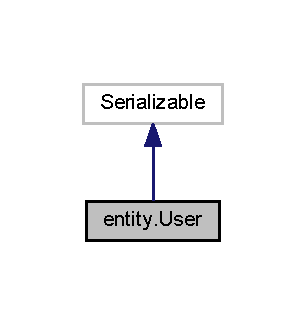
\includegraphics[width=147pt]{classentity_1_1_user__inherit__graph}
\end{center}
\end{figure}


Collaboration diagram for entity.\+User\+:\nopagebreak
\begin{figure}[H]
\begin{center}
\leavevmode
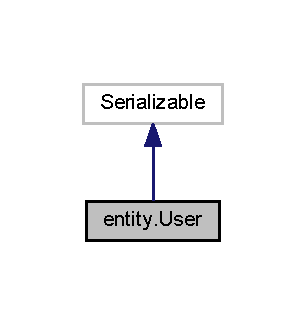
\includegraphics[width=147pt]{classentity_1_1_user__coll__graph}
\end{center}
\end{figure}
\subsection*{Public Member Functions}
\begin{DoxyCompactItemize}
\item 
\mbox{\Hypertarget{classentity_1_1_user_a930c504e6004ddb37035544fbd904166}\label{classentity_1_1_user_a930c504e6004ddb37035544fbd904166}} 
{\bfseries User} (String username, String password, String name, String surname, String mail)
\item 
\mbox{\Hypertarget{classentity_1_1_user_a030c1335a60b60d90e731b1438292d3b}\label{classentity_1_1_user_a030c1335a60b60d90e731b1438292d3b}} 
{\bfseries User} (\mbox{\hyperlink{classentity_1_1_usertype}{Usertype}} usertype, String username, String password, String name, String surname, String mail, Date born\+Dat)
\item 
\mbox{\Hypertarget{classentity_1_1_user_a4004338c97a54b7a80369b5aad8fad0f}\label{classentity_1_1_user_a4004338c97a54b7a80369b5aad8fad0f}} 
int {\bfseries get\+User\+Id} ()
\item 
\mbox{\Hypertarget{classentity_1_1_user_a58e8f4d8e357810b972d52dc1383013e}\label{classentity_1_1_user_a58e8f4d8e357810b972d52dc1383013e}} 
void {\bfseries set\+User\+Id} (int user\+Id)
\item 
\mbox{\Hypertarget{classentity_1_1_user_a050e73c7a9b10da8cec45c60afe9b942}\label{classentity_1_1_user_a050e73c7a9b10da8cec45c60afe9b942}} 
\mbox{\hyperlink{classentity_1_1_usertype}{Usertype}} {\bfseries get\+Usertype} ()
\item 
\mbox{\Hypertarget{classentity_1_1_user_a0981e69a22d9baed58f63d8e757ae7a7}\label{classentity_1_1_user_a0981e69a22d9baed58f63d8e757ae7a7}} 
void {\bfseries set\+Usertype} (\mbox{\hyperlink{classentity_1_1_usertype}{Usertype}} usertype)
\item 
\mbox{\Hypertarget{classentity_1_1_user_a346d96c8b90b4ba0446170f2bf913be8}\label{classentity_1_1_user_a346d96c8b90b4ba0446170f2bf913be8}} 
String {\bfseries get\+Username} ()
\item 
\mbox{\Hypertarget{classentity_1_1_user_a1b88018038c39d85b2e500f5134ca7c5}\label{classentity_1_1_user_a1b88018038c39d85b2e500f5134ca7c5}} 
void {\bfseries set\+Username} (String username)
\item 
\mbox{\Hypertarget{classentity_1_1_user_ac45f7a1da720c4bcc21ce365c29a74b4}\label{classentity_1_1_user_ac45f7a1da720c4bcc21ce365c29a74b4}} 
String {\bfseries get\+Password} ()
\item 
\mbox{\Hypertarget{classentity_1_1_user_a91eda90caa1220f6b2c0ec4aebbf6810}\label{classentity_1_1_user_a91eda90caa1220f6b2c0ec4aebbf6810}} 
void {\bfseries set\+Password} (String password)
\item 
\mbox{\Hypertarget{classentity_1_1_user_aadec9c3bcce34926a4e3dfe092499934}\label{classentity_1_1_user_aadec9c3bcce34926a4e3dfe092499934}} 
String {\bfseries get\+Name} ()
\item 
\mbox{\Hypertarget{classentity_1_1_user_afd002543b54320b13cb004b909083ce4}\label{classentity_1_1_user_afd002543b54320b13cb004b909083ce4}} 
void {\bfseries set\+Name} (String name)
\item 
\mbox{\Hypertarget{classentity_1_1_user_abc6c40b85eae27cc9ce6ff127767b47d}\label{classentity_1_1_user_abc6c40b85eae27cc9ce6ff127767b47d}} 
String {\bfseries get\+Surname} ()
\item 
\mbox{\Hypertarget{classentity_1_1_user_ad4d2d21374dd1352fe8d4d4349dbec0f}\label{classentity_1_1_user_ad4d2d21374dd1352fe8d4d4349dbec0f}} 
void {\bfseries set\+Surname} (String surname)
\item 
\mbox{\Hypertarget{classentity_1_1_user_ab5992e6dcc7b2cd7cf6a03b13b5ffa18}\label{classentity_1_1_user_ab5992e6dcc7b2cd7cf6a03b13b5ffa18}} 
String {\bfseries get\+Mail} ()
\item 
\mbox{\Hypertarget{classentity_1_1_user_a0b95b72010c13f08b795c04165ab4d5c}\label{classentity_1_1_user_a0b95b72010c13f08b795c04165ab4d5c}} 
void {\bfseries set\+Mail} (String mail)
\item 
\mbox{\Hypertarget{classentity_1_1_user_a6252395eaeb3df00686043ccabe886f4}\label{classentity_1_1_user_a6252395eaeb3df00686043ccabe886f4}} 
Date {\bfseries get\+Born\+Dat} ()
\item 
\mbox{\Hypertarget{classentity_1_1_user_af06d5955e7b981aba4858413817e422e}\label{classentity_1_1_user_af06d5955e7b981aba4858413817e422e}} 
void {\bfseries set\+Born\+Dat} (Date born\+Dat)
\item 
\mbox{\Hypertarget{classentity_1_1_user_a415c9d1d1003fb50953170650a8b369f}\label{classentity_1_1_user_a415c9d1d1003fb50953170650a8b369f}} 
String {\bfseries to\+String} ()
\end{DoxyCompactItemize}


\subsection{Detailed Description}
\mbox{\hyperlink{classentity_1_1_user}{User}} generated by hbm2java 

The documentation for this class was generated from the following file\+:\begin{DoxyCompactItemize}
\item 
src/main/java/entity/User.\+java\end{DoxyCompactItemize}

\hypertarget{classrepository_1_1_user_repository}{}\section{repository.\+User\+Repository Class Reference}
\label{classrepository_1_1_user_repository}\index{repository.\+User\+Repository@{repository.\+User\+Repository}}
\subsection*{Public Member Functions}
\begin{DoxyCompactItemize}
\item 
\mbox{\hyperlink{classentity_1_1_user}{User}} \mbox{\hyperlink{classrepository_1_1_user_repository_adf10692a176bf2819fb70895530ef086}{check\+User}} (String uname, String password)
\item 
\mbox{\hyperlink{classentity_1_1_usertype}{Usertype}} \mbox{\hyperlink{classrepository_1_1_user_repository_a8e4a797c0eb806d34793295af70fd281}{check\+Usertype}} (\mbox{\hyperlink{classentity_1_1_user}{User}} user)
\item 
\mbox{\hyperlink{classentity_1_1_usertype}{Usertype}} \mbox{\hyperlink{classrepository_1_1_user_repository_a7da3f6411186e8169f5730638e6a4032}{get\+Usertype\+By\+Id}} (int id)
\item 
\mbox{\hyperlink{classentity_1_1_order}{Order}} \mbox{[}$\,$\mbox{]} \mbox{\hyperlink{classrepository_1_1_user_repository_a56980daa937375f2c13ceb712a08aace}{get\+All\+Orders}} (\mbox{\hyperlink{classentity_1_1_user}{User}} user)
\item 
\mbox{\hyperlink{classentity_1_1_order}{Order}} \mbox{\hyperlink{classrepository_1_1_user_repository_a487c490af80c0a94477bfcfdbe7d288f}{find\+Order\+By\+Id}} (int id)
\item 
List$<$ \mbox{\hyperlink{classentity_1_1_product}{Product}} $>$ \mbox{\hyperlink{classrepository_1_1_user_repository_a413de9a5357ced95cfe6524c47b98bee}{get\+Products\+From\+Order}} (int id)
\item 
\mbox{\hyperlink{classentity_1_1_product}{Product}} \mbox{[}$\,$\mbox{]} \mbox{\hyperlink{classrepository_1_1_user_repository_a91aaaa79a8c1be15fc6111a9467c981e}{get\+All\+Products}} ()
\end{DoxyCompactItemize}


\subsection{Detailed Description}
User Repository. Contains sql queries to get information from database.

\begin{DoxyAuthor}{Author}
Leire 
\end{DoxyAuthor}


\subsection{Member Function Documentation}
\mbox{\Hypertarget{classrepository_1_1_user_repository_adf10692a176bf2819fb70895530ef086}\label{classrepository_1_1_user_repository_adf10692a176bf2819fb70895530ef086}} 
\index{repository\+::\+User\+Repository@{repository\+::\+User\+Repository}!check\+User@{check\+User}}
\index{check\+User@{check\+User}!repository\+::\+User\+Repository@{repository\+::\+User\+Repository}}
\subsubsection{\texorpdfstring{check\+User()}{checkUser()}}
{\footnotesize\ttfamily \mbox{\hyperlink{classentity_1_1_user}{User}} repository.\+User\+Repository.\+check\+User (\begin{DoxyParamCaption}\item[{String}]{uname,  }\item[{String}]{password }\end{DoxyParamCaption})\hspace{0.3cm}{\ttfamily [inline]}}

This method will check a user and its password on the database \mbox{\Hypertarget{classrepository_1_1_user_repository_a8e4a797c0eb806d34793295af70fd281}\label{classrepository_1_1_user_repository_a8e4a797c0eb806d34793295af70fd281}} 
\index{repository\+::\+User\+Repository@{repository\+::\+User\+Repository}!check\+Usertype@{check\+Usertype}}
\index{check\+Usertype@{check\+Usertype}!repository\+::\+User\+Repository@{repository\+::\+User\+Repository}}
\subsubsection{\texorpdfstring{check\+Usertype()}{checkUsertype()}}
{\footnotesize\ttfamily \mbox{\hyperlink{classentity_1_1_usertype}{Usertype}} repository.\+User\+Repository.\+check\+Usertype (\begin{DoxyParamCaption}\item[{\mbox{\hyperlink{classentity_1_1_user}{User}}}]{user }\end{DoxyParamCaption})\hspace{0.3cm}{\ttfamily [inline]}}

This method will return the usertype of the user given \mbox{\Hypertarget{classrepository_1_1_user_repository_a487c490af80c0a94477bfcfdbe7d288f}\label{classrepository_1_1_user_repository_a487c490af80c0a94477bfcfdbe7d288f}} 
\index{repository\+::\+User\+Repository@{repository\+::\+User\+Repository}!find\+Order\+By\+Id@{find\+Order\+By\+Id}}
\index{find\+Order\+By\+Id@{find\+Order\+By\+Id}!repository\+::\+User\+Repository@{repository\+::\+User\+Repository}}
\subsubsection{\texorpdfstring{find\+Order\+By\+Id()}{findOrderById()}}
{\footnotesize\ttfamily \mbox{\hyperlink{classentity_1_1_order}{Order}} repository.\+User\+Repository.\+find\+Order\+By\+Id (\begin{DoxyParamCaption}\item[{int}]{id }\end{DoxyParamCaption})\hspace{0.3cm}{\ttfamily [inline]}}

This method will find an order by its ID \mbox{\Hypertarget{classrepository_1_1_user_repository_a56980daa937375f2c13ceb712a08aace}\label{classrepository_1_1_user_repository_a56980daa937375f2c13ceb712a08aace}} 
\index{repository\+::\+User\+Repository@{repository\+::\+User\+Repository}!get\+All\+Orders@{get\+All\+Orders}}
\index{get\+All\+Orders@{get\+All\+Orders}!repository\+::\+User\+Repository@{repository\+::\+User\+Repository}}
\subsubsection{\texorpdfstring{get\+All\+Orders()}{getAllOrders()}}
{\footnotesize\ttfamily \mbox{\hyperlink{classentity_1_1_order}{Order}} \mbox{[}$\,$\mbox{]} repository.\+User\+Repository.\+get\+All\+Orders (\begin{DoxyParamCaption}\item[{\mbox{\hyperlink{classentity_1_1_user}{User}}}]{user }\end{DoxyParamCaption})\hspace{0.3cm}{\ttfamily [inline]}}

This method will return all the orders of the user given \mbox{\Hypertarget{classrepository_1_1_user_repository_a91aaaa79a8c1be15fc6111a9467c981e}\label{classrepository_1_1_user_repository_a91aaaa79a8c1be15fc6111a9467c981e}} 
\index{repository\+::\+User\+Repository@{repository\+::\+User\+Repository}!get\+All\+Products@{get\+All\+Products}}
\index{get\+All\+Products@{get\+All\+Products}!repository\+::\+User\+Repository@{repository\+::\+User\+Repository}}
\subsubsection{\texorpdfstring{get\+All\+Products()}{getAllProducts()}}
{\footnotesize\ttfamily \mbox{\hyperlink{classentity_1_1_product}{Product}} \mbox{[}$\,$\mbox{]} repository.\+User\+Repository.\+get\+All\+Products (\begin{DoxyParamCaption}{ }\end{DoxyParamCaption})\hspace{0.3cm}{\ttfamily [inline]}}

This method will creturn all the products available \mbox{\Hypertarget{classrepository_1_1_user_repository_a413de9a5357ced95cfe6524c47b98bee}\label{classrepository_1_1_user_repository_a413de9a5357ced95cfe6524c47b98bee}} 
\index{repository\+::\+User\+Repository@{repository\+::\+User\+Repository}!get\+Products\+From\+Order@{get\+Products\+From\+Order}}
\index{get\+Products\+From\+Order@{get\+Products\+From\+Order}!repository\+::\+User\+Repository@{repository\+::\+User\+Repository}}
\subsubsection{\texorpdfstring{get\+Products\+From\+Order()}{getProductsFromOrder()}}
{\footnotesize\ttfamily List$<$\mbox{\hyperlink{classentity_1_1_product}{Product}}$>$ repository.\+User\+Repository.\+get\+Products\+From\+Order (\begin{DoxyParamCaption}\item[{int}]{id }\end{DoxyParamCaption})\hspace{0.3cm}{\ttfamily [inline]}}

This method will find an order by its ID \mbox{\Hypertarget{classrepository_1_1_user_repository_a7da3f6411186e8169f5730638e6a4032}\label{classrepository_1_1_user_repository_a7da3f6411186e8169f5730638e6a4032}} 
\index{repository\+::\+User\+Repository@{repository\+::\+User\+Repository}!get\+Usertype\+By\+Id@{get\+Usertype\+By\+Id}}
\index{get\+Usertype\+By\+Id@{get\+Usertype\+By\+Id}!repository\+::\+User\+Repository@{repository\+::\+User\+Repository}}
\subsubsection{\texorpdfstring{get\+Usertype\+By\+Id()}{getUsertypeById()}}
{\footnotesize\ttfamily \mbox{\hyperlink{classentity_1_1_usertype}{Usertype}} repository.\+User\+Repository.\+get\+Usertype\+By\+Id (\begin{DoxyParamCaption}\item[{int}]{id }\end{DoxyParamCaption})\hspace{0.3cm}{\ttfamily [inline]}}

This method will find a user and return its type 

The documentation for this class was generated from the following file\+:\begin{DoxyCompactItemize}
\item 
D\+:/\+Users/user/\+Documents/\+M\+O\+N\+D\+R\+A/3.\+M\+A\+I\+L\+A/\+P\+O\+P\+B\+L5/\+G\+I\+T/e\+Jkiva\+\_\+\+P\+O\+P\+B\+L5/e\+Jkiva/src/main/java/repository/User\+Repository.\+java\end{DoxyCompactItemize}

\hypertarget{classentity_1_1_usertype}{}\section{entity.\+Usertype Class Reference}
\label{classentity_1_1_usertype}\index{entity.\+Usertype@{entity.\+Usertype}}


Inheritance diagram for entity.\+Usertype\+:\nopagebreak
\begin{figure}[H]
\begin{center}
\leavevmode
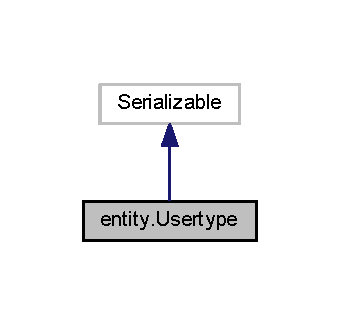
\includegraphics[width=163pt]{classentity_1_1_usertype__inherit__graph}
\end{center}
\end{figure}


Collaboration diagram for entity.\+Usertype\+:\nopagebreak
\begin{figure}[H]
\begin{center}
\leavevmode
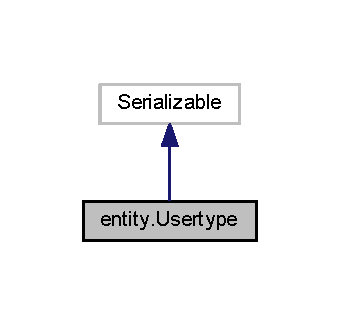
\includegraphics[width=163pt]{classentity_1_1_usertype__coll__graph}
\end{center}
\end{figure}
\subsection*{Public Member Functions}
\begin{DoxyCompactItemize}
\item 
\mbox{\Hypertarget{classentity_1_1_usertype_a3f17f72e004920b8d0099586a5b016fe}\label{classentity_1_1_usertype_a3f17f72e004920b8d0099586a5b016fe}} 
{\bfseries Usertype} (String usertype)
\item 
\mbox{\Hypertarget{classentity_1_1_usertype_aa9776ce9c7de7443a232c0531d78ea8b}\label{classentity_1_1_usertype_aa9776ce9c7de7443a232c0531d78ea8b}} 
{\bfseries Usertype} (String usertype, String description)
\item 
\mbox{\Hypertarget{classentity_1_1_usertype_a361cfd2f23d71f1ec7e69aa55e5f013c}\label{classentity_1_1_usertype_a361cfd2f23d71f1ec7e69aa55e5f013c}} 
int {\bfseries get\+Usertype\+Id} ()
\item 
\mbox{\Hypertarget{classentity_1_1_usertype_ad05f418dbd08027c7afac5e4af7d2254}\label{classentity_1_1_usertype_ad05f418dbd08027c7afac5e4af7d2254}} 
void {\bfseries set\+Usertype\+Id} (int usertype\+Id)
\item 
\mbox{\Hypertarget{classentity_1_1_usertype_ad300a2783e57d8690d9db0c3b464737b}\label{classentity_1_1_usertype_ad300a2783e57d8690d9db0c3b464737b}} 
String {\bfseries get\+Usertype} ()
\item 
\mbox{\Hypertarget{classentity_1_1_usertype_ac4220b848c369fd726b0c8bebc8dbcf3}\label{classentity_1_1_usertype_ac4220b848c369fd726b0c8bebc8dbcf3}} 
void {\bfseries set\+Usertype} (String usertype)
\item 
\mbox{\Hypertarget{classentity_1_1_usertype_a1699b78e303deb9b70224bf863b08063}\label{classentity_1_1_usertype_a1699b78e303deb9b70224bf863b08063}} 
String {\bfseries get\+Description} ()
\item 
\mbox{\Hypertarget{classentity_1_1_usertype_ab274da7bcfaa15606599fc856b958d24}\label{classentity_1_1_usertype_ab274da7bcfaa15606599fc856b958d24}} 
void {\bfseries set\+Description} (String description)
\item 
\mbox{\Hypertarget{classentity_1_1_usertype_a4211735d5a357a4dbd778c1b1aa4b7e0}\label{classentity_1_1_usertype_a4211735d5a357a4dbd778c1b1aa4b7e0}} 
String {\bfseries to\+String} ()
\end{DoxyCompactItemize}


\subsection{Detailed Description}
\mbox{\hyperlink{classentity_1_1_usertype}{Usertype}} generated by hbm2java 

The documentation for this class was generated from the following file\+:\begin{DoxyCompactItemize}
\item 
src/main/java/entity/Usertype.\+java\end{DoxyCompactItemize}

\hypertarget{classentity_1_1copy_1_1_usertype}{}\section{entity.\+copy.\+Usertype Class Reference}
\label{classentity_1_1copy_1_1_usertype}\index{entity.\+copy.\+Usertype@{entity.\+copy.\+Usertype}}


Inheritance diagram for entity.\+copy.\+Usertype\+:
% FIG 0


Collaboration diagram for entity.\+copy.\+Usertype\+:
% FIG 1
\subsection*{Public Member Functions}
\begin{DoxyCompactItemize}
\item 
\mbox{\Hypertarget{classentity_1_1copy_1_1_usertype_ac3ce0ce958d0c3bea17d240edbac174e}\label{classentity_1_1copy_1_1_usertype_ac3ce0ce958d0c3bea17d240edbac174e}} 
{\bfseries Usertype} (String usertype)
\item 
\mbox{\Hypertarget{classentity_1_1copy_1_1_usertype_a61039f08470265f57f229ffe16086de9}\label{classentity_1_1copy_1_1_usertype_a61039f08470265f57f229ffe16086de9}} 
{\bfseries Usertype} (String usertype, String description)
\item 
\mbox{\Hypertarget{classentity_1_1copy_1_1_usertype_ab9650d3e80eafd3630f1b9eeb7c30fb0}\label{classentity_1_1copy_1_1_usertype_ab9650d3e80eafd3630f1b9eeb7c30fb0}} 
int {\bfseries get\+Usertype\+Id} ()
\item 
\mbox{\Hypertarget{classentity_1_1copy_1_1_usertype_a282dc800f5c063117f514a8d143da70f}\label{classentity_1_1copy_1_1_usertype_a282dc800f5c063117f514a8d143da70f}} 
void {\bfseries set\+Usertype\+Id} (int usertype\+Id)
\item 
\mbox{\Hypertarget{classentity_1_1copy_1_1_usertype_a52ee6376362ddf89577bf45afc6d24a4}\label{classentity_1_1copy_1_1_usertype_a52ee6376362ddf89577bf45afc6d24a4}} 
String {\bfseries get\+Usertype} ()
\item 
\mbox{\Hypertarget{classentity_1_1copy_1_1_usertype_a2d6d1c8e6c10b354c99bc322e4de6a93}\label{classentity_1_1copy_1_1_usertype_a2d6d1c8e6c10b354c99bc322e4de6a93}} 
void {\bfseries set\+Usertype} (String usertype)
\item 
\mbox{\Hypertarget{classentity_1_1copy_1_1_usertype_a1b1461147a837afc5089c3c877fb10e9}\label{classentity_1_1copy_1_1_usertype_a1b1461147a837afc5089c3c877fb10e9}} 
String {\bfseries get\+Description} ()
\item 
\mbox{\Hypertarget{classentity_1_1copy_1_1_usertype_a63c9c8b5f7fe4a39cb4788e94e4d66ca}\label{classentity_1_1copy_1_1_usertype_a63c9c8b5f7fe4a39cb4788e94e4d66ca}} 
void {\bfseries set\+Description} (String description)
\item 
\mbox{\Hypertarget{classentity_1_1copy_1_1_usertype_a8036d5139f37b27e90cbed19ec8749bc}\label{classentity_1_1copy_1_1_usertype_a8036d5139f37b27e90cbed19ec8749bc}} 
String {\bfseries to\+String} ()
\end{DoxyCompactItemize}


\subsection{Detailed Description}
\mbox{\hyperlink{classentity_1_1copy_1_1_usertype}{Usertype}} generated by hbm2java 

The documentation for this class was generated from the following file\+:\begin{DoxyCompactItemize}
\item 
D\+:/\+Users/user/\+Documents/\+M\+O\+N\+D\+R\+A/3.\+M\+A\+I\+L\+A/\+P\+O\+P\+B\+L5/\+G\+I\+T/e\+Jkiva\+\_\+\+P\+O\+P\+B\+L5/e\+Jkiva/src/main/java/entity/copy/Usertype.\+java\end{DoxyCompactItemize}

\hypertarget{classentity_1_1_workstation}{}\section{entity.\+Workstation Class Reference}
\label{classentity_1_1_workstation}\index{entity.\+Workstation@{entity.\+Workstation}}


Inheritance diagram for entity.\+Workstation\+:
% FIG 0


Collaboration diagram for entity.\+Workstation\+:
% FIG 1
\subsection*{Public Member Functions}
\begin{DoxyCompactItemize}
\item 
\mbox{\Hypertarget{classentity_1_1_workstation_a377e0a2bbe7044cc7f486bae0ea8ed67}\label{classentity_1_1_workstation_a377e0a2bbe7044cc7f486bae0ea8ed67}} 
{\bfseries Workstation} (String workstation\+Nam)
\item 
\mbox{\Hypertarget{classentity_1_1_workstation_a22288e3495ba499b6bde23eb07f7101b}\label{classentity_1_1_workstation_a22288e3495ba499b6bde23eb07f7101b}} 
{\bfseries Workstation} (\mbox{\hyperlink{classentity_1_1_segment}{Segment}} segment, String workstation\+Nam, String description, Boolean state, Set carrieses\+For\+Destiny\+Workstation\+Id, Set carrieses\+For\+Initial\+Workstation\+Id)
\item 
\mbox{\Hypertarget{classentity_1_1_workstation_abb73425f42c9c651fdd58e06e9dd5e8b}\label{classentity_1_1_workstation_abb73425f42c9c651fdd58e06e9dd5e8b}} 
int {\bfseries get\+Workstation\+Id} ()
\item 
\mbox{\Hypertarget{classentity_1_1_workstation_a34dbc056f3a0bfa3a94aebfc8a0f0d68}\label{classentity_1_1_workstation_a34dbc056f3a0bfa3a94aebfc8a0f0d68}} 
void {\bfseries set\+Workstation\+Id} (int workstation\+Id)
\item 
\mbox{\Hypertarget{classentity_1_1_workstation_a41f03757564ca8adcdc0a062c33f99d4}\label{classentity_1_1_workstation_a41f03757564ca8adcdc0a062c33f99d4}} 
\mbox{\hyperlink{classentity_1_1_segment}{Segment}} {\bfseries get\+Segment} ()
\item 
\mbox{\Hypertarget{classentity_1_1_workstation_a419f3d517914ff99b9c3b1a151deaf37}\label{classentity_1_1_workstation_a419f3d517914ff99b9c3b1a151deaf37}} 
void {\bfseries set\+Segment} (\mbox{\hyperlink{classentity_1_1_segment}{Segment}} segment)
\item 
\mbox{\Hypertarget{classentity_1_1_workstation_a8af3245910985e27ce7e8d5d1acd3e2d}\label{classentity_1_1_workstation_a8af3245910985e27ce7e8d5d1acd3e2d}} 
String {\bfseries get\+Workstation\+Nam} ()
\item 
\mbox{\Hypertarget{classentity_1_1_workstation_ae21df43c124cfd95deb4845726473b19}\label{classentity_1_1_workstation_ae21df43c124cfd95deb4845726473b19}} 
void {\bfseries set\+Workstation\+Nam} (String workstation\+Nam)
\item 
\mbox{\Hypertarget{classentity_1_1_workstation_ae79cd9019eb03d8526727c98ade26905}\label{classentity_1_1_workstation_ae79cd9019eb03d8526727c98ade26905}} 
String {\bfseries get\+Description} ()
\item 
\mbox{\Hypertarget{classentity_1_1_workstation_ad164f196f2a925758dac0e9b9e28484b}\label{classentity_1_1_workstation_ad164f196f2a925758dac0e9b9e28484b}} 
void {\bfseries set\+Description} (String description)
\item 
\mbox{\Hypertarget{classentity_1_1_workstation_a49be3c2bef3d42a5596844c603712061}\label{classentity_1_1_workstation_a49be3c2bef3d42a5596844c603712061}} 
Boolean {\bfseries get\+State} ()
\item 
\mbox{\Hypertarget{classentity_1_1_workstation_a33d712bc34bd23dcf56492d3dd562635}\label{classentity_1_1_workstation_a33d712bc34bd23dcf56492d3dd562635}} 
void {\bfseries set\+State} (Boolean state)
\item 
\mbox{\Hypertarget{classentity_1_1_workstation_a0da8d108a3195e74a9cd37a48ac80e0d}\label{classentity_1_1_workstation_a0da8d108a3195e74a9cd37a48ac80e0d}} 
Set {\bfseries get\+Carrieses\+For\+Destiny\+Workstation\+Id} ()
\item 
\mbox{\Hypertarget{classentity_1_1_workstation_a9d7abfff67413a398a7927928caa8f35}\label{classentity_1_1_workstation_a9d7abfff67413a398a7927928caa8f35}} 
void {\bfseries set\+Carrieses\+For\+Destiny\+Workstation\+Id} (Set carrieses\+For\+Destiny\+Workstation\+Id)
\item 
\mbox{\Hypertarget{classentity_1_1_workstation_a9cc802a3b25ea2b483b776ccd0f4a24a}\label{classentity_1_1_workstation_a9cc802a3b25ea2b483b776ccd0f4a24a}} 
Set {\bfseries get\+Carrieses\+For\+Initial\+Workstation\+Id} ()
\item 
\mbox{\Hypertarget{classentity_1_1_workstation_a5ac57917431af5a9a85ada5a74f7c64e}\label{classentity_1_1_workstation_a5ac57917431af5a9a85ada5a74f7c64e}} 
void {\bfseries set\+Carrieses\+For\+Initial\+Workstation\+Id} (Set carrieses\+For\+Initial\+Workstation\+Id)
\end{DoxyCompactItemize}


\subsection{Detailed Description}
\mbox{\hyperlink{classentity_1_1_workstation}{Workstation}} generated by hbm2java 

The documentation for this class was generated from the following file\+:\begin{DoxyCompactItemize}
\item 
D\+:/\+Users/user/\+Documents/\+M\+O\+N\+D\+R\+A/3.\+M\+A\+I\+L\+A/\+P\+O\+P\+B\+L5/\+G\+I\+T/e\+Jkiva\+\_\+\+P\+O\+P\+B\+L5/e\+Jkiva/src/main/java/entity/Workstation.\+java\end{DoxyCompactItemize}

\hypertarget{classentity_1_1copy_1_1_workstation}{}\section{entity.\+copy.\+Workstation Class Reference}
\label{classentity_1_1copy_1_1_workstation}\index{entity.\+copy.\+Workstation@{entity.\+copy.\+Workstation}}


Inheritance diagram for entity.\+copy.\+Workstation\+:
% FIG 0


Collaboration diagram for entity.\+copy.\+Workstation\+:
% FIG 1
\subsection*{Public Member Functions}
\begin{DoxyCompactItemize}
\item 
\mbox{\Hypertarget{classentity_1_1copy_1_1_workstation_a448c76d94800dcc1b179daf2856084ef}\label{classentity_1_1copy_1_1_workstation_a448c76d94800dcc1b179daf2856084ef}} 
{\bfseries Workstation} (String workstation\+Nam)
\item 
\mbox{\Hypertarget{classentity_1_1copy_1_1_workstation_a0ae93ddf50a960b83e8b73f90a3b6405}\label{classentity_1_1copy_1_1_workstation_a0ae93ddf50a960b83e8b73f90a3b6405}} 
{\bfseries Workstation} (\mbox{\hyperlink{classentity_1_1copy_1_1_segment}{Segment}} segment, String workstation\+Nam, String description, Boolean state, Set carrieses\+For\+Destiny\+Workstation\+Id, Set carrieses\+For\+Initial\+Workstation\+Id)
\item 
\mbox{\Hypertarget{classentity_1_1copy_1_1_workstation_abbdfa8113fbe3f99fe86961a9b94aac7}\label{classentity_1_1copy_1_1_workstation_abbdfa8113fbe3f99fe86961a9b94aac7}} 
int {\bfseries get\+Workstation\+Id} ()
\item 
\mbox{\Hypertarget{classentity_1_1copy_1_1_workstation_a46c647486665990074a8426f66c9b175}\label{classentity_1_1copy_1_1_workstation_a46c647486665990074a8426f66c9b175}} 
void {\bfseries set\+Workstation\+Id} (int workstation\+Id)
\item 
\mbox{\Hypertarget{classentity_1_1copy_1_1_workstation_a3d829847163d15c627e8bc0c81a8537e}\label{classentity_1_1copy_1_1_workstation_a3d829847163d15c627e8bc0c81a8537e}} 
\mbox{\hyperlink{classentity_1_1copy_1_1_segment}{Segment}} {\bfseries get\+Segment} ()
\item 
\mbox{\Hypertarget{classentity_1_1copy_1_1_workstation_aa848584af51a84c21e2e7e9662a5391a}\label{classentity_1_1copy_1_1_workstation_aa848584af51a84c21e2e7e9662a5391a}} 
void {\bfseries set\+Segment} (\mbox{\hyperlink{classentity_1_1copy_1_1_segment}{Segment}} segment)
\item 
\mbox{\Hypertarget{classentity_1_1copy_1_1_workstation_aed94d2ada3c15744e8a80d722493bdea}\label{classentity_1_1copy_1_1_workstation_aed94d2ada3c15744e8a80d722493bdea}} 
String {\bfseries get\+Workstation\+Nam} ()
\item 
\mbox{\Hypertarget{classentity_1_1copy_1_1_workstation_ae8325bcb478ba2b217283e36a0fc7040}\label{classentity_1_1copy_1_1_workstation_ae8325bcb478ba2b217283e36a0fc7040}} 
void {\bfseries set\+Workstation\+Nam} (String workstation\+Nam)
\item 
\mbox{\Hypertarget{classentity_1_1copy_1_1_workstation_adf871ad7a5cc25a555a3fe52d9352515}\label{classentity_1_1copy_1_1_workstation_adf871ad7a5cc25a555a3fe52d9352515}} 
String {\bfseries get\+Description} ()
\item 
\mbox{\Hypertarget{classentity_1_1copy_1_1_workstation_a6eb07774bbfade50adc81f5114a0ea75}\label{classentity_1_1copy_1_1_workstation_a6eb07774bbfade50adc81f5114a0ea75}} 
void {\bfseries set\+Description} (String description)
\item 
\mbox{\Hypertarget{classentity_1_1copy_1_1_workstation_a006351c895b27595c477034925351f5b}\label{classentity_1_1copy_1_1_workstation_a006351c895b27595c477034925351f5b}} 
Boolean {\bfseries get\+State} ()
\item 
\mbox{\Hypertarget{classentity_1_1copy_1_1_workstation_a2d393d110a694567d3615b004562da77}\label{classentity_1_1copy_1_1_workstation_a2d393d110a694567d3615b004562da77}} 
void {\bfseries set\+State} (Boolean state)
\item 
\mbox{\Hypertarget{classentity_1_1copy_1_1_workstation_a03bc877808e7e887f4c797f0b65f3c9b}\label{classentity_1_1copy_1_1_workstation_a03bc877808e7e887f4c797f0b65f3c9b}} 
Set {\bfseries get\+Carrieses\+For\+Destiny\+Workstation\+Id} ()
\item 
\mbox{\Hypertarget{classentity_1_1copy_1_1_workstation_ac81c43d28440e0f47ca840728a207ce3}\label{classentity_1_1copy_1_1_workstation_ac81c43d28440e0f47ca840728a207ce3}} 
void {\bfseries set\+Carrieses\+For\+Destiny\+Workstation\+Id} (Set carrieses\+For\+Destiny\+Workstation\+Id)
\item 
\mbox{\Hypertarget{classentity_1_1copy_1_1_workstation_ae47801761c012db3977af32352f860a4}\label{classentity_1_1copy_1_1_workstation_ae47801761c012db3977af32352f860a4}} 
Set {\bfseries get\+Carrieses\+For\+Initial\+Workstation\+Id} ()
\item 
\mbox{\Hypertarget{classentity_1_1copy_1_1_workstation_abecb65e6c6e1eae6692d81ebb5acfd93}\label{classentity_1_1copy_1_1_workstation_abecb65e6c6e1eae6692d81ebb5acfd93}} 
void {\bfseries set\+Carrieses\+For\+Initial\+Workstation\+Id} (Set carrieses\+For\+Initial\+Workstation\+Id)
\end{DoxyCompactItemize}


\subsection{Detailed Description}
\mbox{\hyperlink{classentity_1_1copy_1_1_workstation}{Workstation}} generated by hbm2java 

The documentation for this class was generated from the following file\+:\begin{DoxyCompactItemize}
\item 
D\+:/\+Users/user/\+Documents/\+M\+O\+N\+D\+R\+A/3.\+M\+A\+I\+L\+A/\+P\+O\+P\+B\+L5/\+G\+I\+T/e\+Jkiva\+\_\+\+P\+O\+P\+B\+L5/e\+Jkiva/src/main/java/entity/copy/Workstation.\+java\end{DoxyCompactItemize}

%--- End generated contents ---

% Index
\backmatter
\newpage
\phantomsection
\clearemptydoublepage
\addcontentsline{toc}{chapter}{Index}
\printindex

\end{document}
